\chapter{Simulation Study 2}
\label{C:chap_sim3}

This Simulation study again uses the framework described in Chapter \ref{C:chap_sim_design} but compared to Chapter \ref{C:chap_sim2} more complex patterns of treatment effect are considered. The main objective of this simulation study is to investigate the sensitivity of the RPSFT and MIPE methods to violations of the common treatment effect assumption in the presence of correlated survival times.

\section{Study design}

Table \ref{T:chap_sim3:scenarios} shows a summary of the scenarios investigated and parameters for treatment effects (as defined in Chapter \ref{C:chap_sim_design}). For each of the 6 scenarios investigated $\rho$, the correlation between Time to Progression and Overall Survival, is varied across 6 levels from 0 to 1 and the proportion of patients who switch is set at 40\% and 60\% leading to 72 scenarios in total. For each of these 72 scenarios 1000 datasets are simulated. 

\begin{table}[ht] 
\caption{Treatment effect scenarios for simulation study 2}
\centering 
\begin{tabular}{ l l r r r r}
\hline
\hline
Description & ID & \multicolumn{4}{c}{Treatment effects} \\
         &             & \multicolumn{2}{c}{Experimental arm} & \multicolumn{2}{c}{Control arm} \\
%         &             & during    & after      & during     & after     \\
		 &             & $\exp(\beta_{1a})$ & $\exp(\beta_{1b})$ & $\exp(\beta_{2a})$ & $\exp(\beta_{2b})$ \\
\hline
Common effect during treatment      & 1 & $0.5$ & $0.8$ & $0.5$ & $0.8$ \\
with reduced effect after treatment & 2 & $0.8$ & $0.95$ & $0.8$ & $0.95$ \\            
\\
Common effect during treatment     & 3 & $0.01$ & $1$ & $0.01$ & $1$ \\
with no effect after treatment     & 4 & $0.4$  & $1$ & $0.4$ & $1$ \\
\\
Lower effect of switch treatment & 5 & $0.7$ & $0.7$ & $0.8$ & $0.8$ \\
sustained after treatment        & 6 & $0.7$ & $0.7$ & $0.9$ & $0.9$ \\
\hline
\end{tabular} 
\label{T:chap_sim3:scenarios}
\end{table}



\subsection{Rationale for scenarios}

The scenarios 1-4 considered here are meant to represent a treatment effect where a greater reduction on risk of death is received during treatment than after treatment. In scenarios 1 and 2 some residual treatment effect remains after progression and treatment discontinuation whereas for scenarios 3 and 4 there is no residual treatment effect after progression/discontinuation. While at first glance it may appear these scenarios satisfy the common treatment effect assumption of the RPSFT and MIPE method this is not the case as these treatment effects as a reduction in hazard do not translate to a single treatment effect as an acceleration factor. 

Scenarios 5 and 6 are explicitly designed to violate the assumptions of the RPSFT and MIPE approaches in that the treatment benefit received by switch patients are lower than that received by patients receiving randomized treatment. These represent scenarios where patients who have progressed may have a lower capacity to benefit from treatment.

\subsection{Defining a true hazard ratio}


It can be seen that for this simulation study defining the true hazard ratio is problematic for scenarios 1-4 due to the time dependent nature of the treatment effects. To address this the approach of \cite{Latimer2016} is taken and for each of these scenarios 500'000 control and 500'000 experimental patients are generated without switching with the result of this comparison taken as the true value that estimates will be compared against. These ``true'' estimates and the relationship with the correlation between time to progression and overall survival are shown in Figure \ref{F:chap_sim3:truehr}. In these cases what is termed the true hazard ratio is really an average hazard ratio over the observation time of the simulated trial. 

While this approach of defining the ``true'' estimate that the methods are compared against will be prone to some error with the large number of patients used this error should be minimal. A more serious criticism of these scenarios is the use of a Cox model to estimate an average hazard ratio for data where the proportional hazards assumption is clearly violated. Indeed \cite{Schemper1992} show that the Cox model is likely to underestimate the true average hazard ratio in these scenarios even ignoring the problem of treatment switching. Despite this the scenarios are still interesting as what is being examined is how close the proposed methods come to the estimate of hazard ratio that would have been seen without switch. 

\begin{figure}[ht]
\centering
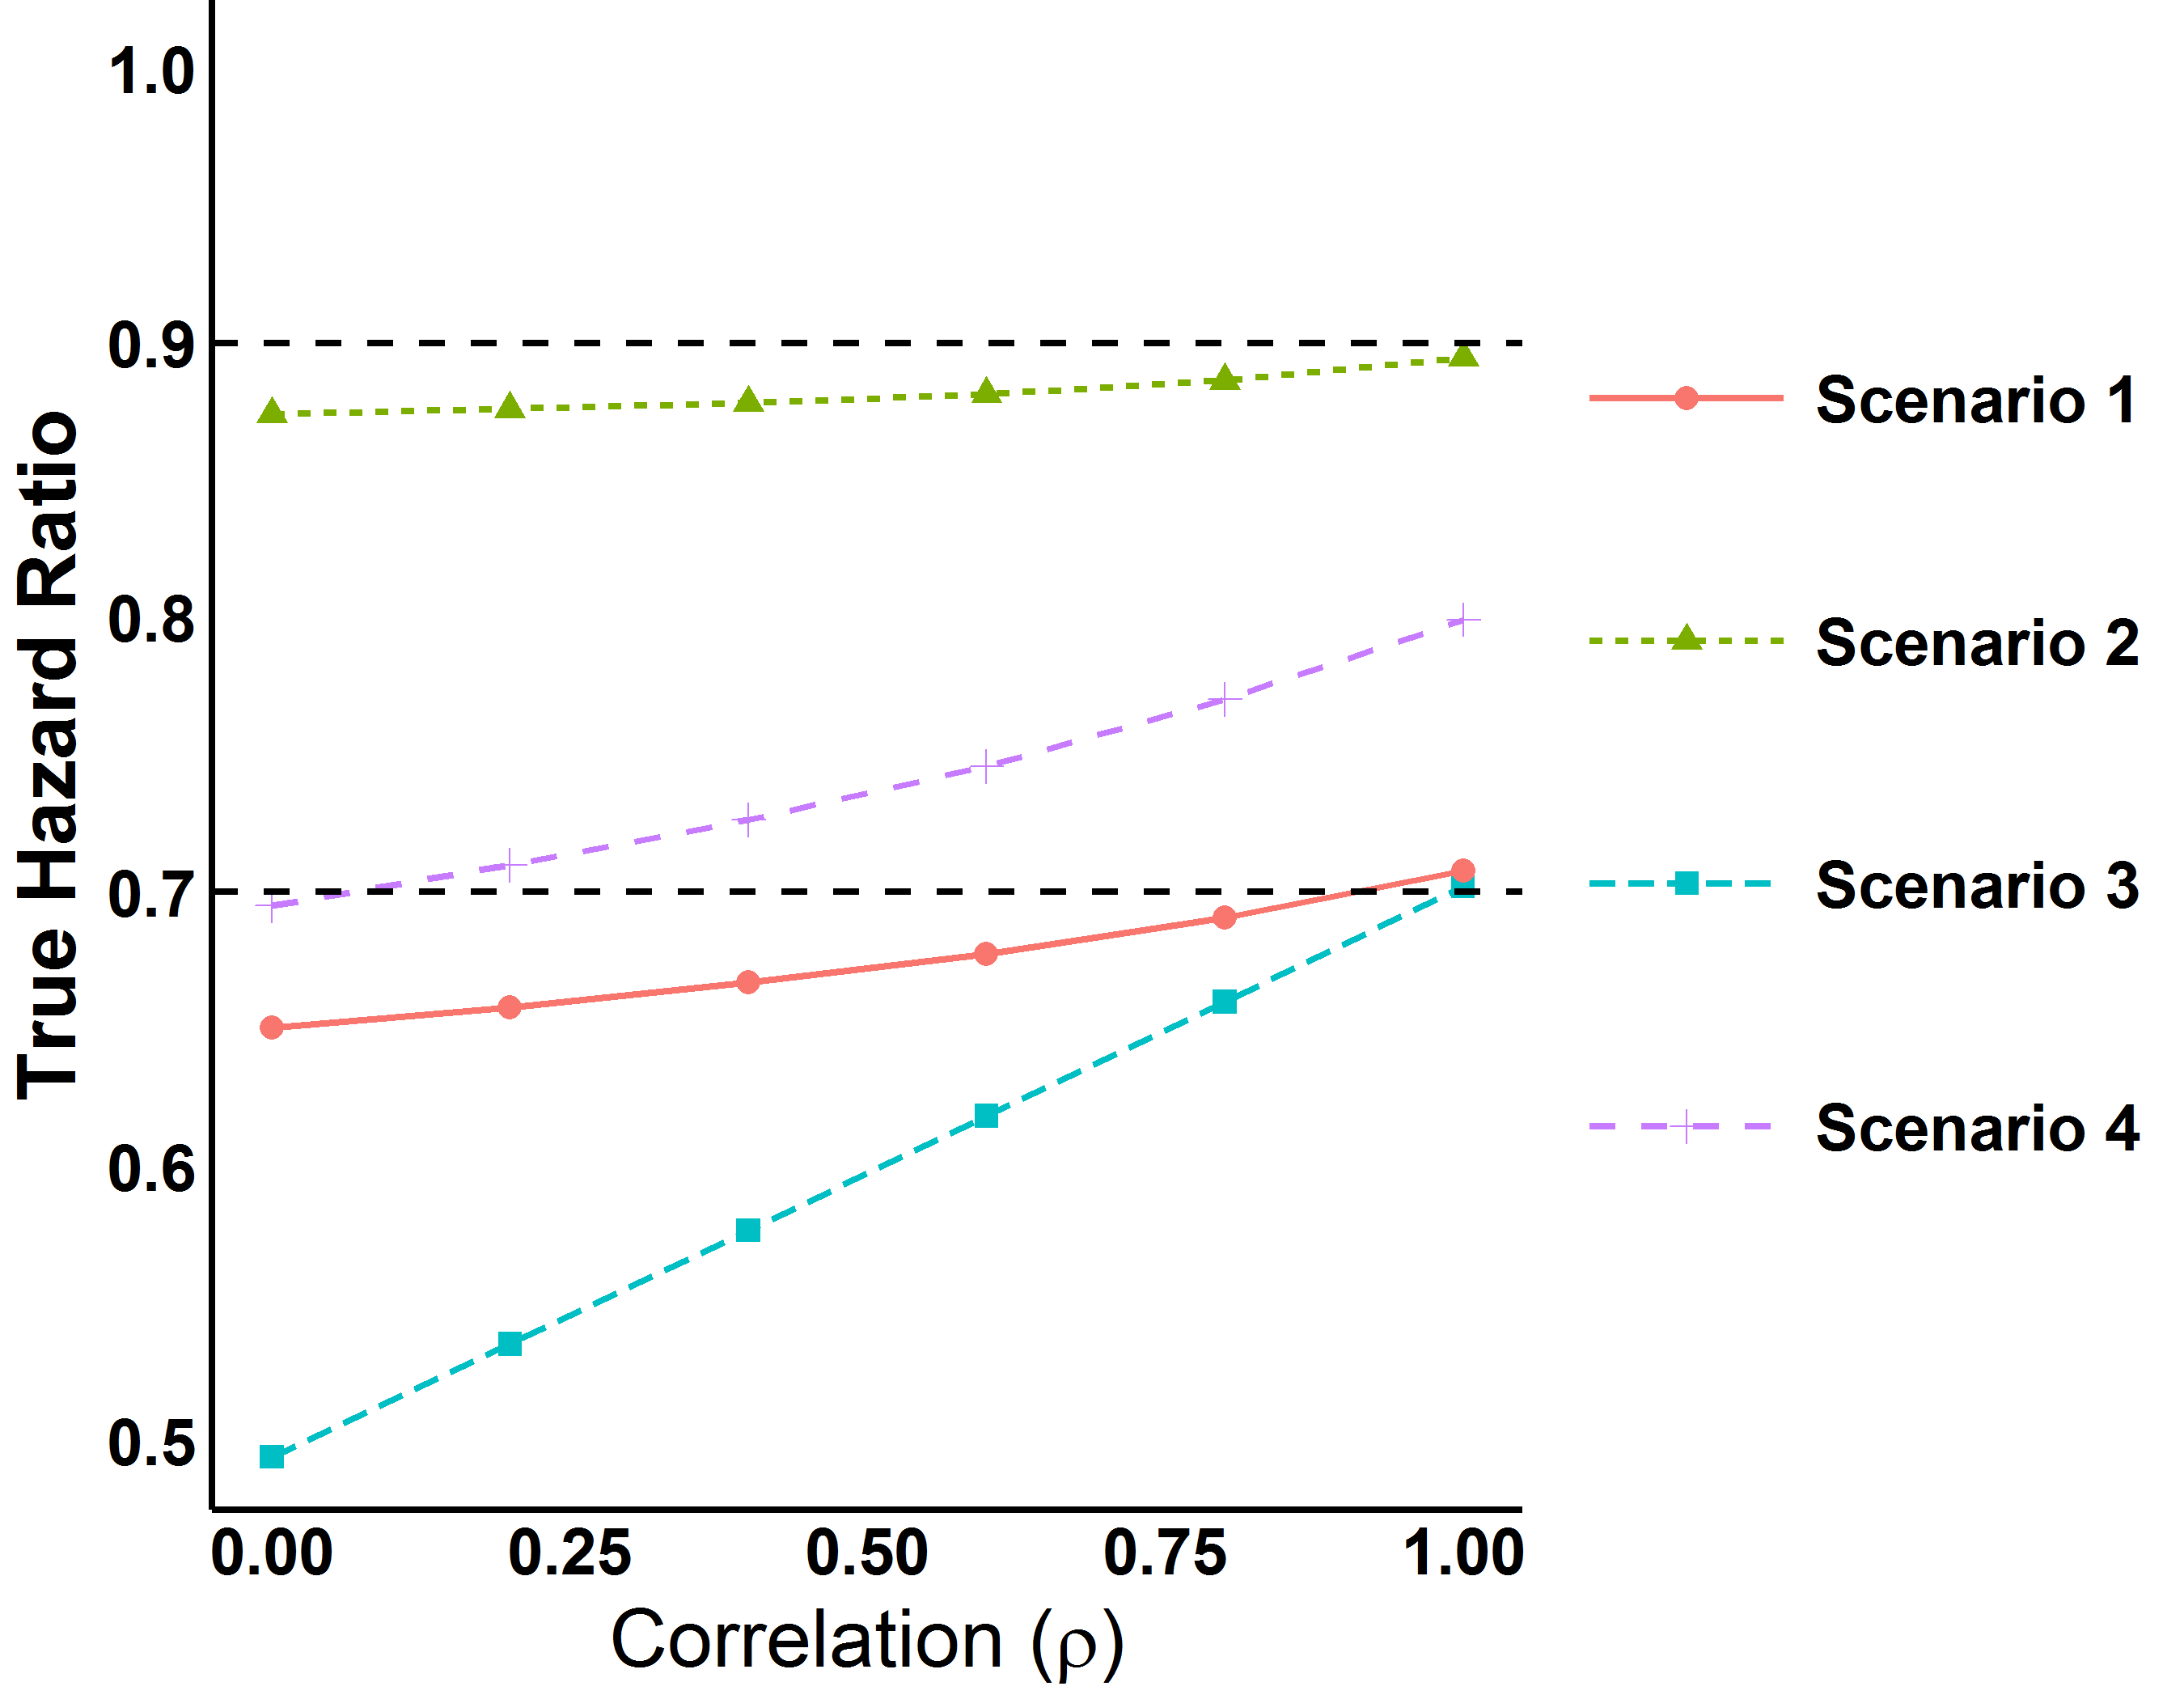
\includegraphics[width=9cm]{images/chap_sim3/truehr.png}
\caption{\label{F:chap_sim3:truehr}  As the application of treatment effects for Scenario 1, 2, 3 and 4 is time dependent the ``true'' average hazard ratio, i.e. that which would be seen if switching did not occur, is estimated using a comparison of 500'000 simulated patients. These average hazard ratios are similar to those simulated in Chapter \ref{C:chap_sim2} as shown by the dashed black lines. The reason the hazard ratio increases with correlation is due to the simulated censoring mechanism whereby patients with the longest simulated overall survival will be often censored when they also receive the longest treatment exposure which is the case when TTP is correlated with OS. } 
\end{figure}

\section{Methods assessed}

The same methods assessed in Chapter \ref{C:chap_sim2} are once again considered and are applied again as described in Section \ref{S:chap_sim2:methass} with the exception that non-convergence of the RPSFT methods is handled differently as described below. 

\subsection{Issues with g-estimation}
\label{S:chap_sim3:gest}
In the previous simulation study the methods described in Section \ref{S:chap_methrev:ESTissues} were used to get an estimate for $\psi$ that is a weighted mean of potential solutions. However, in this simulation study reviewing some plots of the g-estimation procedure for the ``on treatment'' approach to RPSFT suggest this maybe inappropriate with two examples shown in Figure \ref{F:chap_sim3:badgest}. For Example 1 taking a weighted mean as proposed by \cite{White1999} seems reasonable while for Example 2 the range of potential values is so large making such an imputation is questionable. In order to address this I decided to apply a tolerance for convergence whereby if the range of values for $\psi$ where $z(\psi)=0$ were small then the weighted mean would be taken otherwise the simulation would be considered not converged and not analysed. Figure \ref{F:chap_sim3:convcdf} shows the cumulative distribution for convergence across all the scenarios considered. Based on this plot it was decided to allow a tolerance of 0.2 on the range of $\psi$ found for the RPSFT approach with results for this labelled as RPSFT-TOL in all plots and tables.
\begin{figure}[ht]
\centering
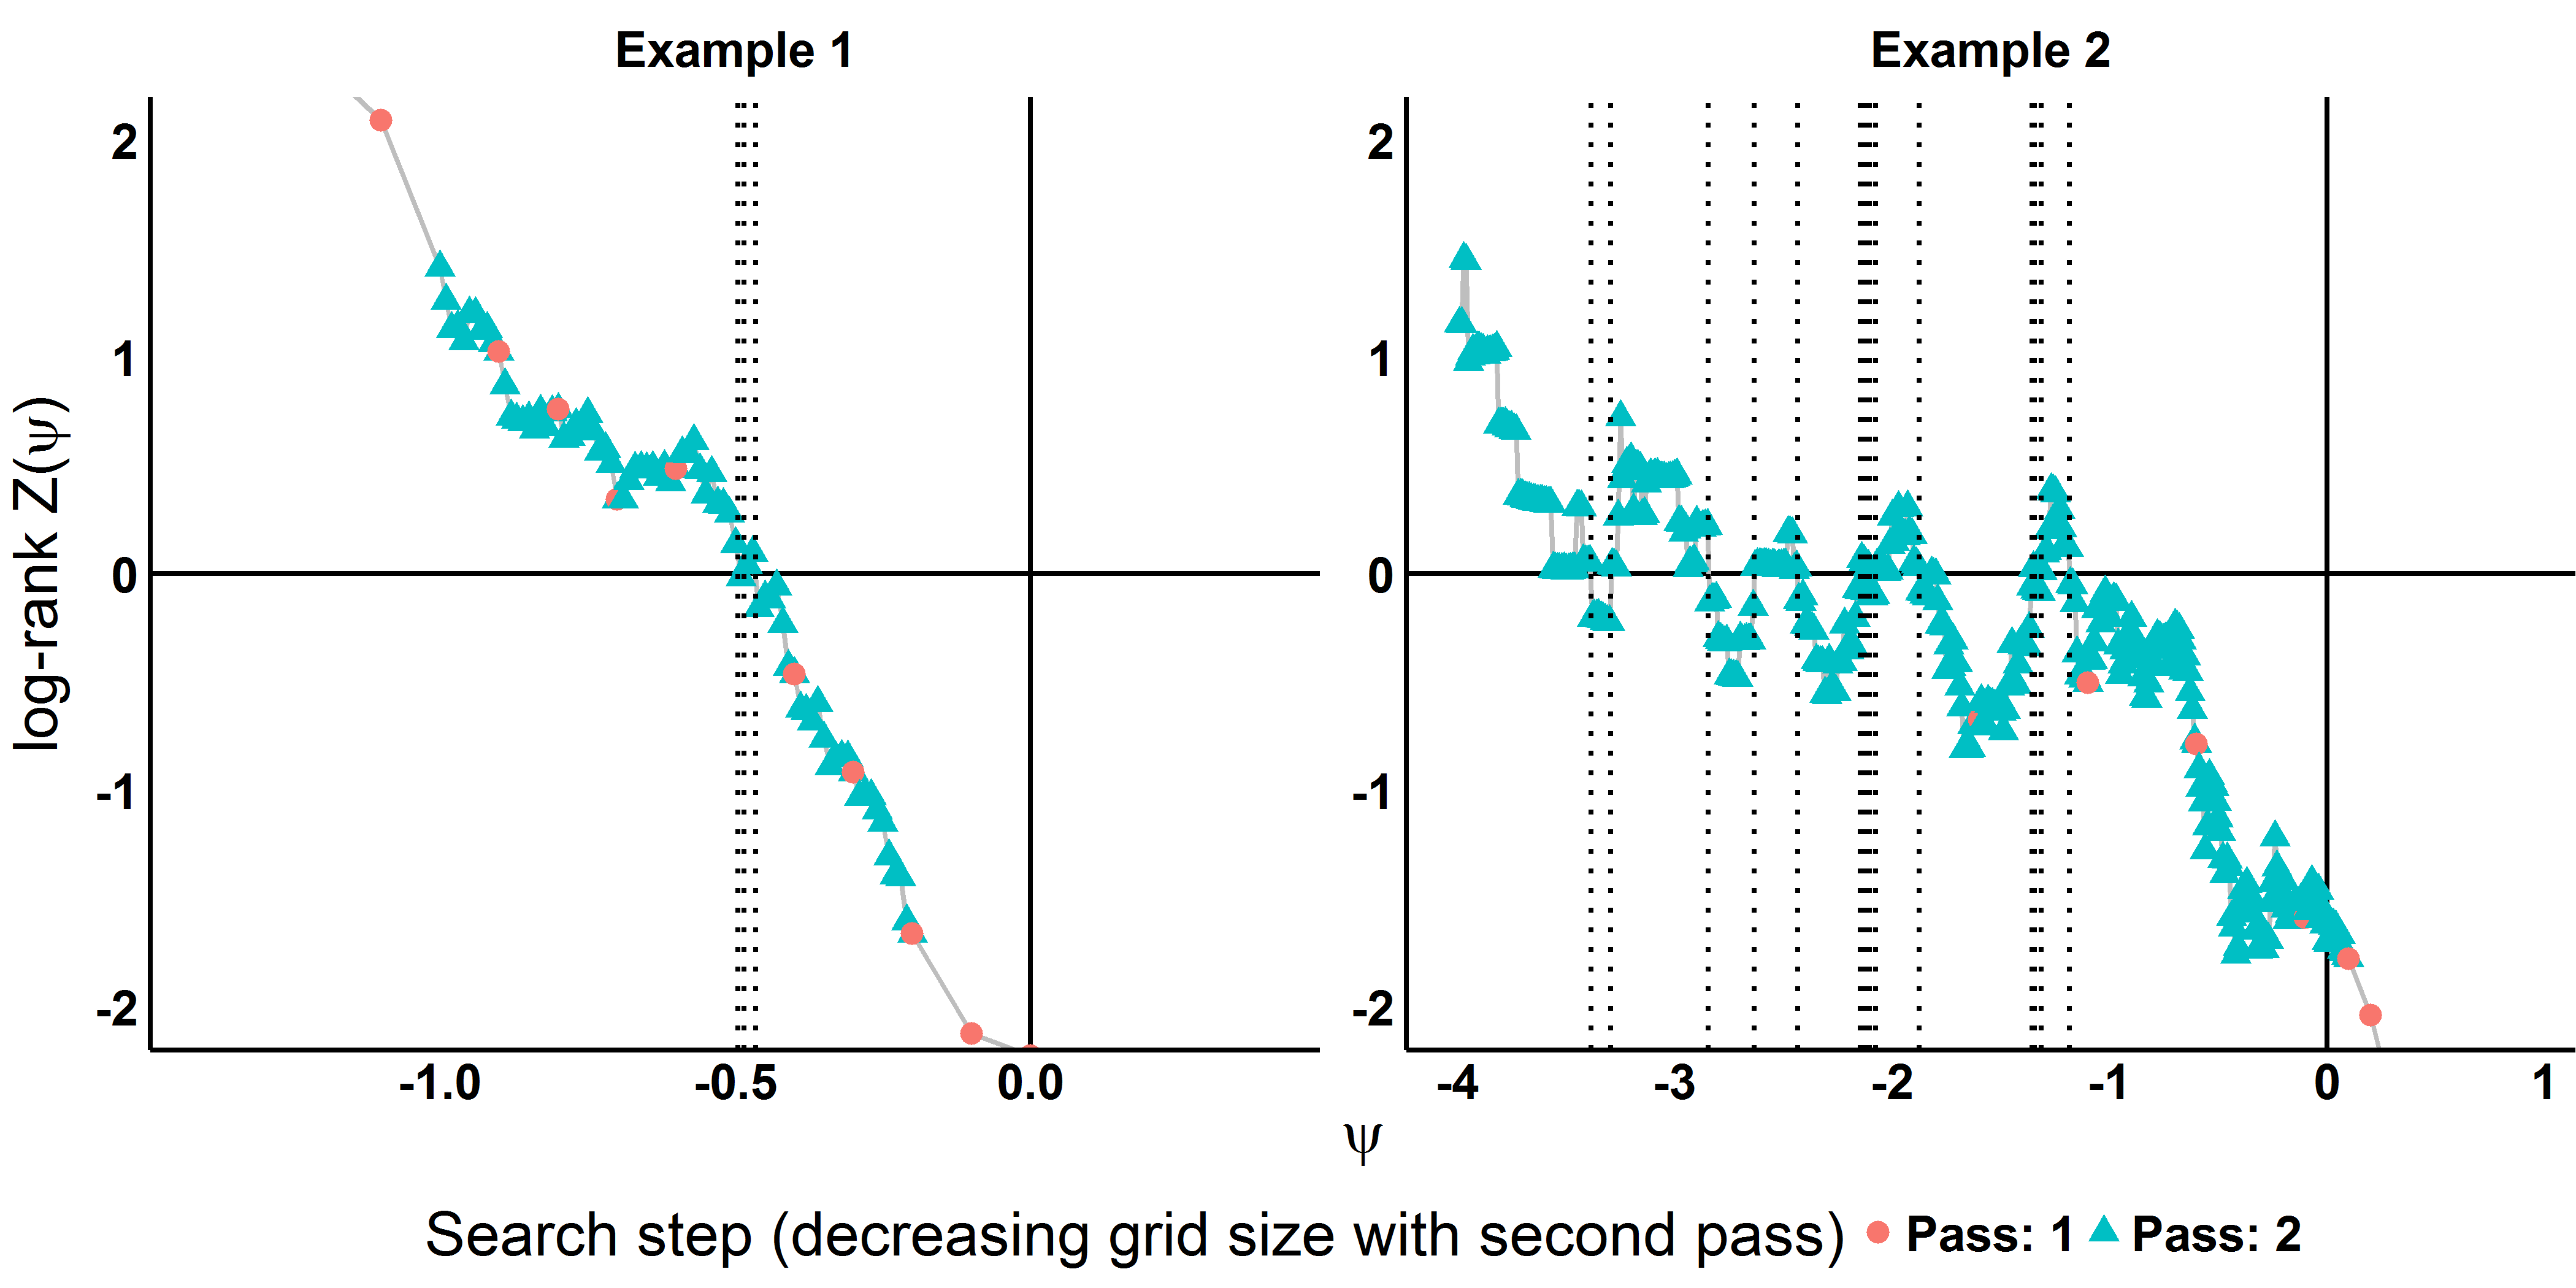
\includegraphics[width=13cm]{images/chap_sim3/badsearch.png}
\caption{\label{F:chap_sim3:badgest} Two examples of problems in g-estimation using log-rank test statistic. In Example 1 the potential values for $\hat{\psi}$ are all quite similar ranging from  $-0.495$ to $-0.465$ while for Example 2 the values where $z(\psi)=0$ range from $-3.385$ to $-1.185$. } 
\end{figure}

\begin{figure}[ht]
\centering
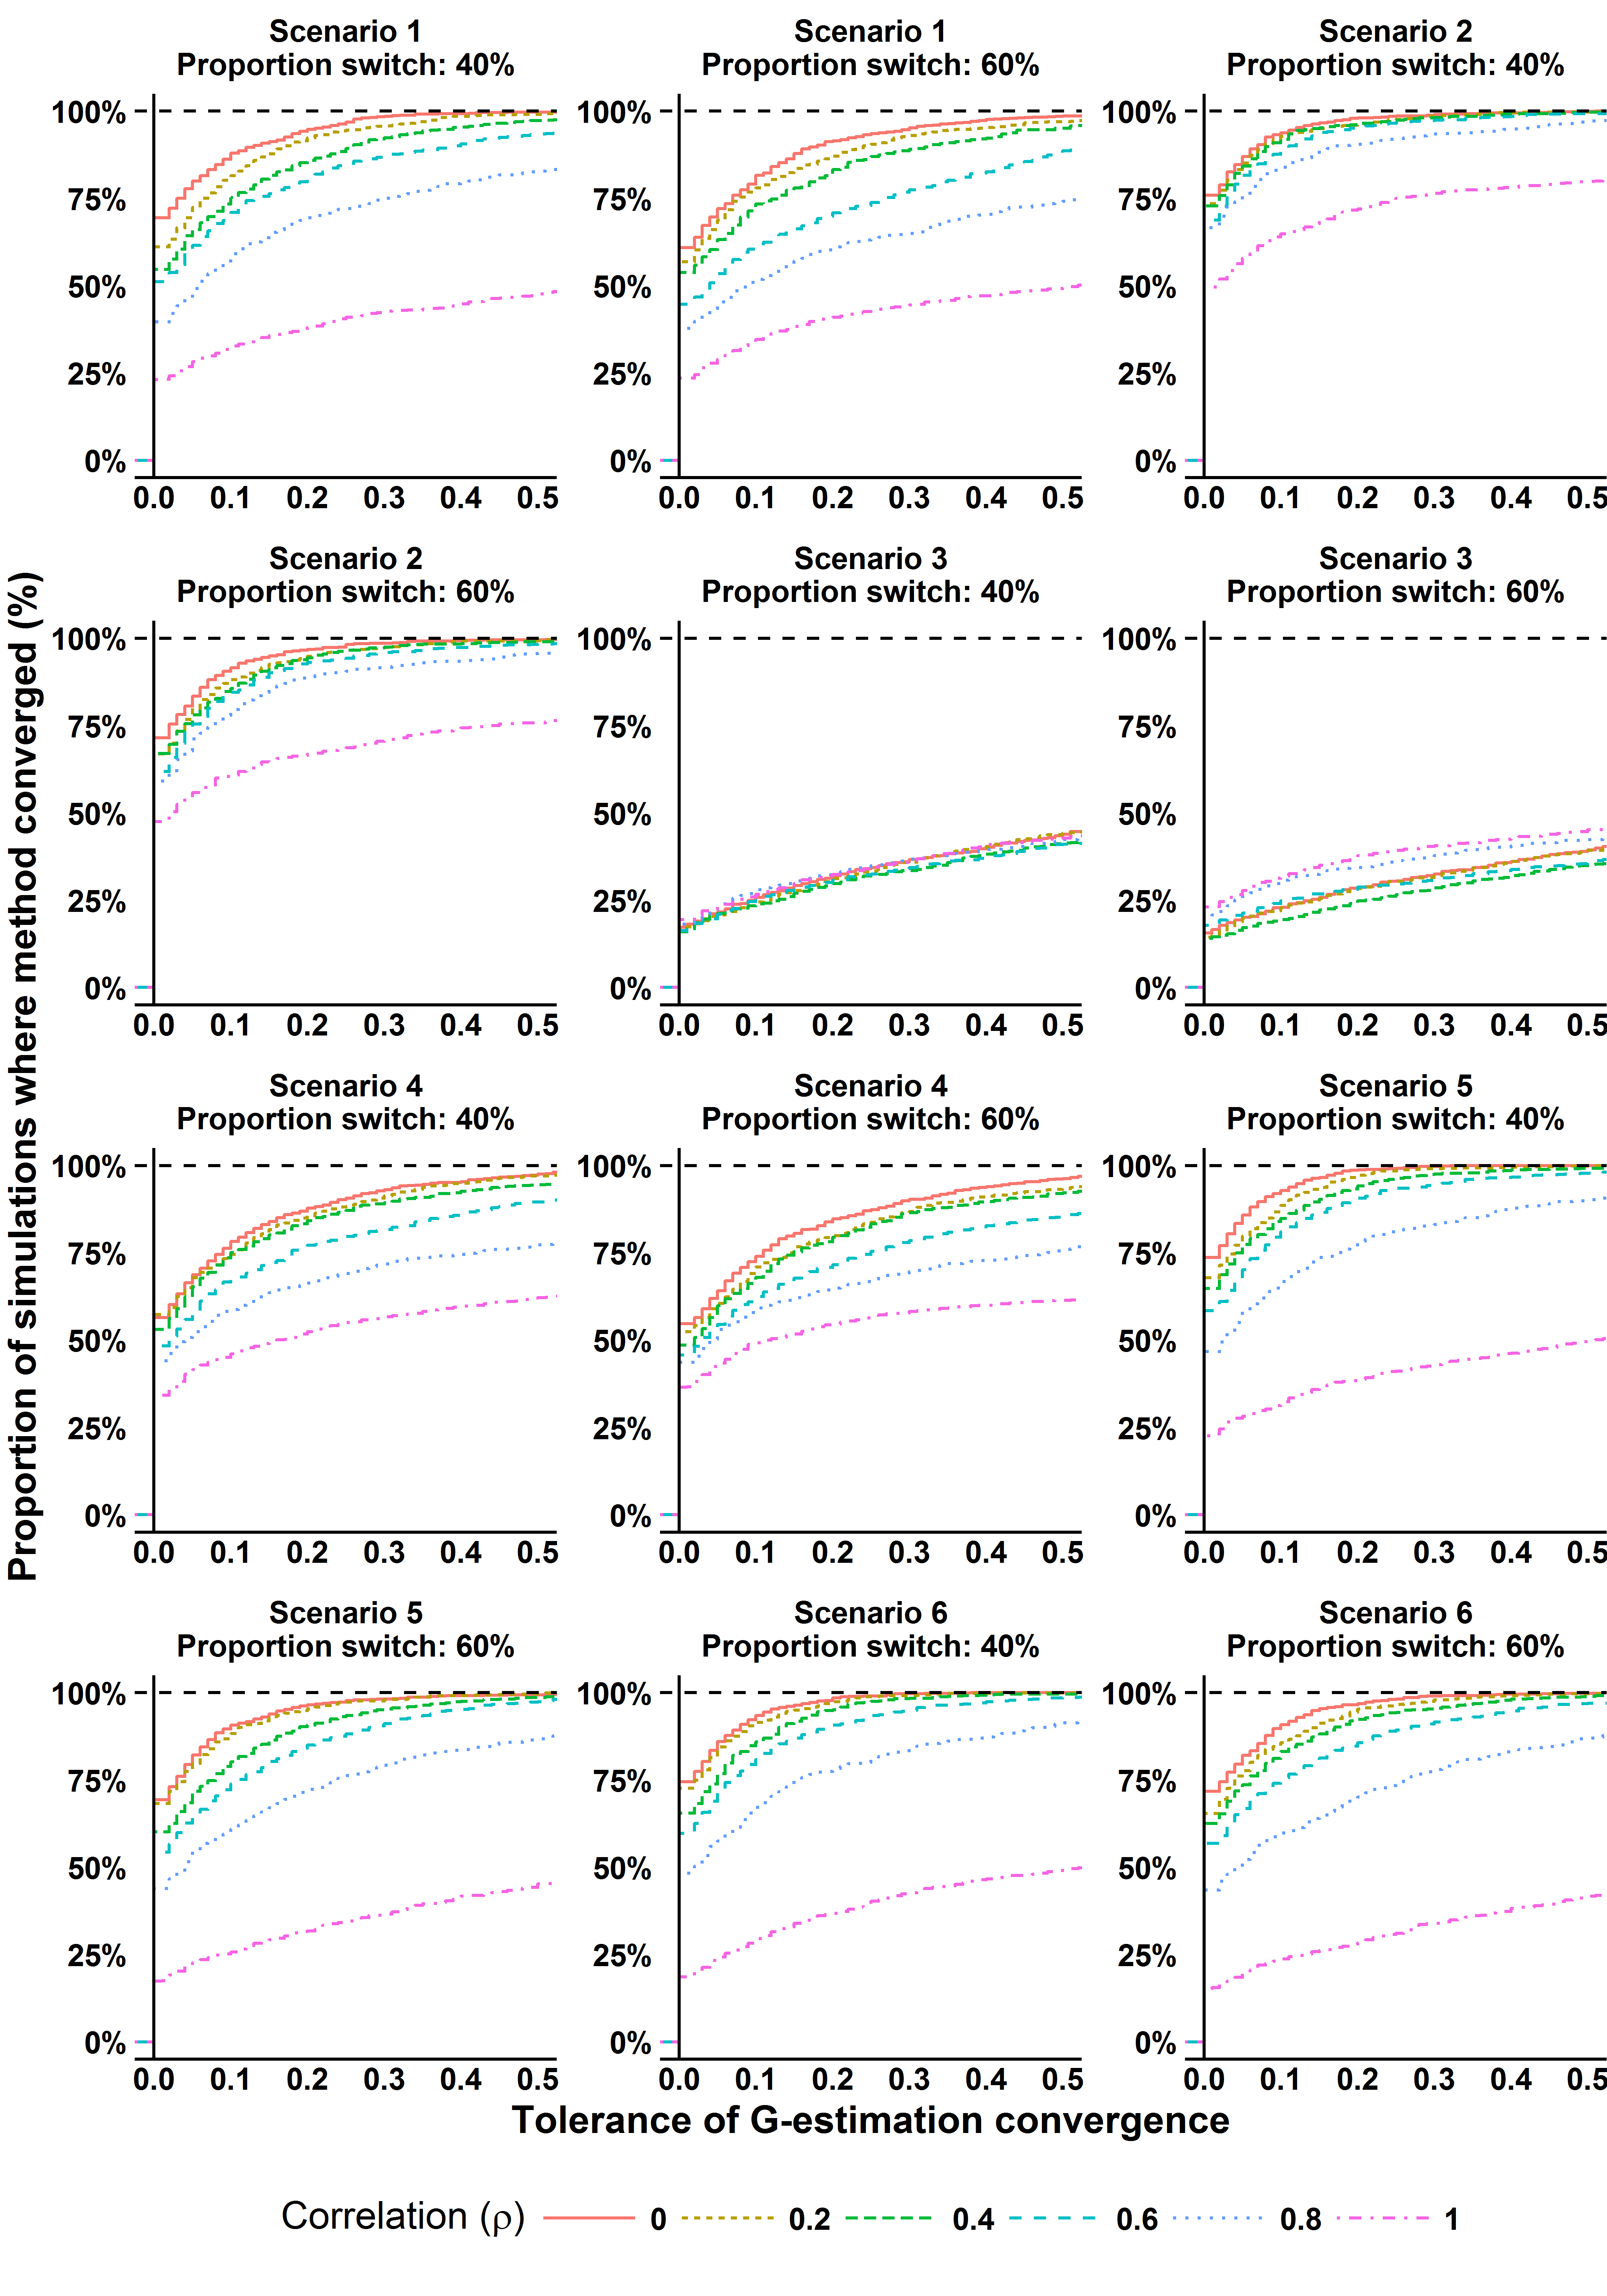
\includegraphics[width=13cm]{images/chap_sim3/conv_cdf.png}
\caption{\label{F:chap_sim3:convcdf}  This figure shows the cumulative distribution of proportion of simulations where the ``on treatment'' approach to rank-preserving failure time (RPSFT) converged for different tolerances on convergence. A tolerance of 0 implies a unique solution was found with increasing tolerance allowing a broader range of multiple solutions for $\psi$ still being considered as converged. Based on this it was decided to investigate further a tolerance of 0.2 in the estimates of $\psi$. Even with this imputation the convergence in Scenario 3 is very poor.} 
\end{figure}

\clearpage

\section{Results}

Table \ref{T:chap_sim3:simres} shows a summary of the results for selected methods grouped by scenario while complete results can be found in Appendix \ref{A:sim3res}. The same methods as discussed in Section \ref{S:chap_sim2:resmeth} are used to assess the methods with the outcome of interest again a hazard ratio for experimental treatment compared to control for overall survival. As with the previous simulation study the results for the RPSFT method using both wilcoxon and log-rank tests in the g-estimation were very similar so only the results using the log-rank test are discussed here.

\begin{table}[ht] 
\caption{The range of bias, MSE, coverage and convergence across scenarios for selected methods\label{T:chap_sim3:simres}}
\centering 
\scalebox{0.9}{
% latex table generated in R 3.3.1 by xtable 1.8-2 package
% Thu Sep 15 18:21:03 2016
\scalebox{0.9}{
\begin{tabular}{lrrrrr}
  \hline
\hline
Scenarios & Method & Bias  & MSE & Coverage & Convergence  \\  &  & $(\%)$ &   & $(\%)$ & $(\%)$ \\  &  & min, max & min, max & min, max & min, max \\ 
  \hline
1 and 2 & ITT &   5.42, 25.54 & 0.02, 0.04 & 66.5, 94.2 & 100.0, 100.0 \\ 
  1 and 2 & PP-CENS &  -1.97, 47.03 & 0.01, 0.23 & 44.0, 95.4 & 100.0, 100.0 \\ 
  1 and 2 & TVC &  -3.02, 75.03 & 0.01, 0.51 &  5.9, 94.9 & 100.0, 100.0 \\ 
  1 and 2 & TVC2 &  -1.89, 56.00 & 0.01, 0.31 & 31.2, 95.4 & 100.0, 100.0 \\ 
  1 and 2 & RPSFT-TG-LR &  -1.09,  8.25 & 0.02, 0.06 & 90.1, 96.1 & 90.6, 99.7 \\ 
  1 and 2 & RPSFT-OT-LR-TU-TOL &  -2.35, 21.12 & 0.03, 0.07 & 74.1, 94.0 & 40.7, 97.9 \\ 
  1 and 2 & RPSFT-OT-LR-V-TOL &  -3.14, 21.11 & 0.03, 0.16 & 85.9, 95.0 & 40.7, 97.9 \\ 
  1 and 2 & 2SAFT &  -3.14,  2.34 & 0.01, 0.03 & 84.5, 95.6 & 100.0, 100.0 \\ 
  1 and 2 & MIPE-ALL & -22.91, -2.60 & 0.05, 0.07 & 43.4, 69.8 & 100.0, 100.0 \\ 
  1 and 2 & MIPE-WEIB &   4.04, 26.12 & 0.03, 0.10 &  & 25.7, 55.4 \\ 
   \hline
3 and 4 & ITT &  11.92, 44.11 & 0.02, 0.07 & 36.2, 86.8 & 100.0, 100.0 \\ 
  3 and 4 & PP-CENS & -10.56, 46.02 & 0.01, 0.18 & 46.6, 96.2 & 100.0, 100.0 \\ 
  3 and 4 & TVC & -14.97, 69.01 & 0.01, 0.35 & 11.1, 96.0 & 100.0, 100.0 \\ 
  3 and 4 & TVC2 & -10.87, 53.93 & 0.01, 0.23 & 33.9, 96.0 & 100.0, 100.0 \\ 
  3 and 4 & RPSFT-TG-LR & -22.72, 17.08 & 0.03, 0.07 & 83.0, 92.9 & 93.5, 99.9 \\ 
  3 and 4 & RPSFT-OT-LR-TU-TOL & -12.72, 35.50 & 0.04, 0.10 & 57.2, 86.3 & 33.4, 87.4 \\ 
  3 and 4 & RPSFT-OT-LR-V-TOL & -13.92, 41.12 & 0.04, 0.20 & 61.8, 89.5 & 33.4, 87.4 \\ 
  3 and 4 & 2SAFT & -24.66,  1.19 & 0.01, 0.03 & 61.6, 95.0 & 100.0, 100.0 \\ 
  3 and 4 & MIPE-ALL & -51.25,  7.60 & 0.05, 0.08 & 14.5, 59.9 & 100.0, 100.0 \\ 
  3 and 4 & MIPE-WEIB & -11.07, 41.90 & 0.02, 0.15 &  & 21.8, 48.8 \\ 
   \hline
5 and 6 & ITT &   3.75,  13.75 & 0.01, 0.02 & 85.5, 95.8 & 100.0, 100.0 \\ 
  5 and 6 & PP-CENS &   0.52,  48.23 & 0.01, 0.15 & 44.6, 95.6 & 100.0, 100.0 \\ 
  5 and 6 & TVC &   4.99,  95.90 & 0.01, 0.50 &  1.7, 95.1 & 100.0, 100.0 \\ 
  5 and 6 & TVC2 &   0.52,  59.28 & 0.01, 0.21 & 26.7, 95.5 & 100.0, 100.0 \\ 
  5 and 6 & RPSFT-TG-LR & -15.61,  -2.60 & 0.02, 0.03 & 87.5, 93.2 & 98.4, 100.0 \\ 
  5 and 6 & RPSFT-OT-LR-TU-TOL & -11.28,   5.77 & 0.02, 0.04 & 80.6, 90.7 & 36.7, 98.6 \\ 
  5 and 6 & RPSFT-OT-LR-V-TOL & -13.97,   3.04 & 0.02, 0.05 & 84.8, 92.9 & 36.7, 98.6 \\ 
  5 and 6 & 2SAFT &  -0.04,   2.62 & 0.01, 0.02 & 86.1, 94.9 & 100.0, 100.0 \\ 
  5 and 6 & MIPE-ALL & -35.27, -21.33 & 0.06, 0.09 & 27.2, 43.9 & 100.0, 100.0 \\ 
  5 and 6 & MIPE-WEIB & -13.93,   4.87 & 0.02, 0.05 &  & 25.1, 31.1 \\ 
   \hline
\end{tabular}
}

}
\end{table}

\clearpage

\subsection{Convergence}

As already discussed in Section \ref{S:chap_sim3:gest} the convergence for the ``on treatment'' approach to RPSFT was poor in this simulation study which can be seen in Figure \ref{F:chap_sim3:conv}. In particular the convergence is lower for higher correlations between time to progression and overall survival. Of interest here is that the ``treatment group'' approach to RPSFT again appears to have no convergence issues and converges to a unique solution much more consistently than the iterative parameter estimation procedure (MIPE). Again as the primary benefit of the iterative parameter estimation method is an improved estimation procedure in exchange for making a parametric assumption on the survival time distribution this is unexpected. Finally the simple methods and the two-stage AFT (2SAFT) converge consistently across all the scenarios investigated. 

\begin{figure}[ht]
\centering
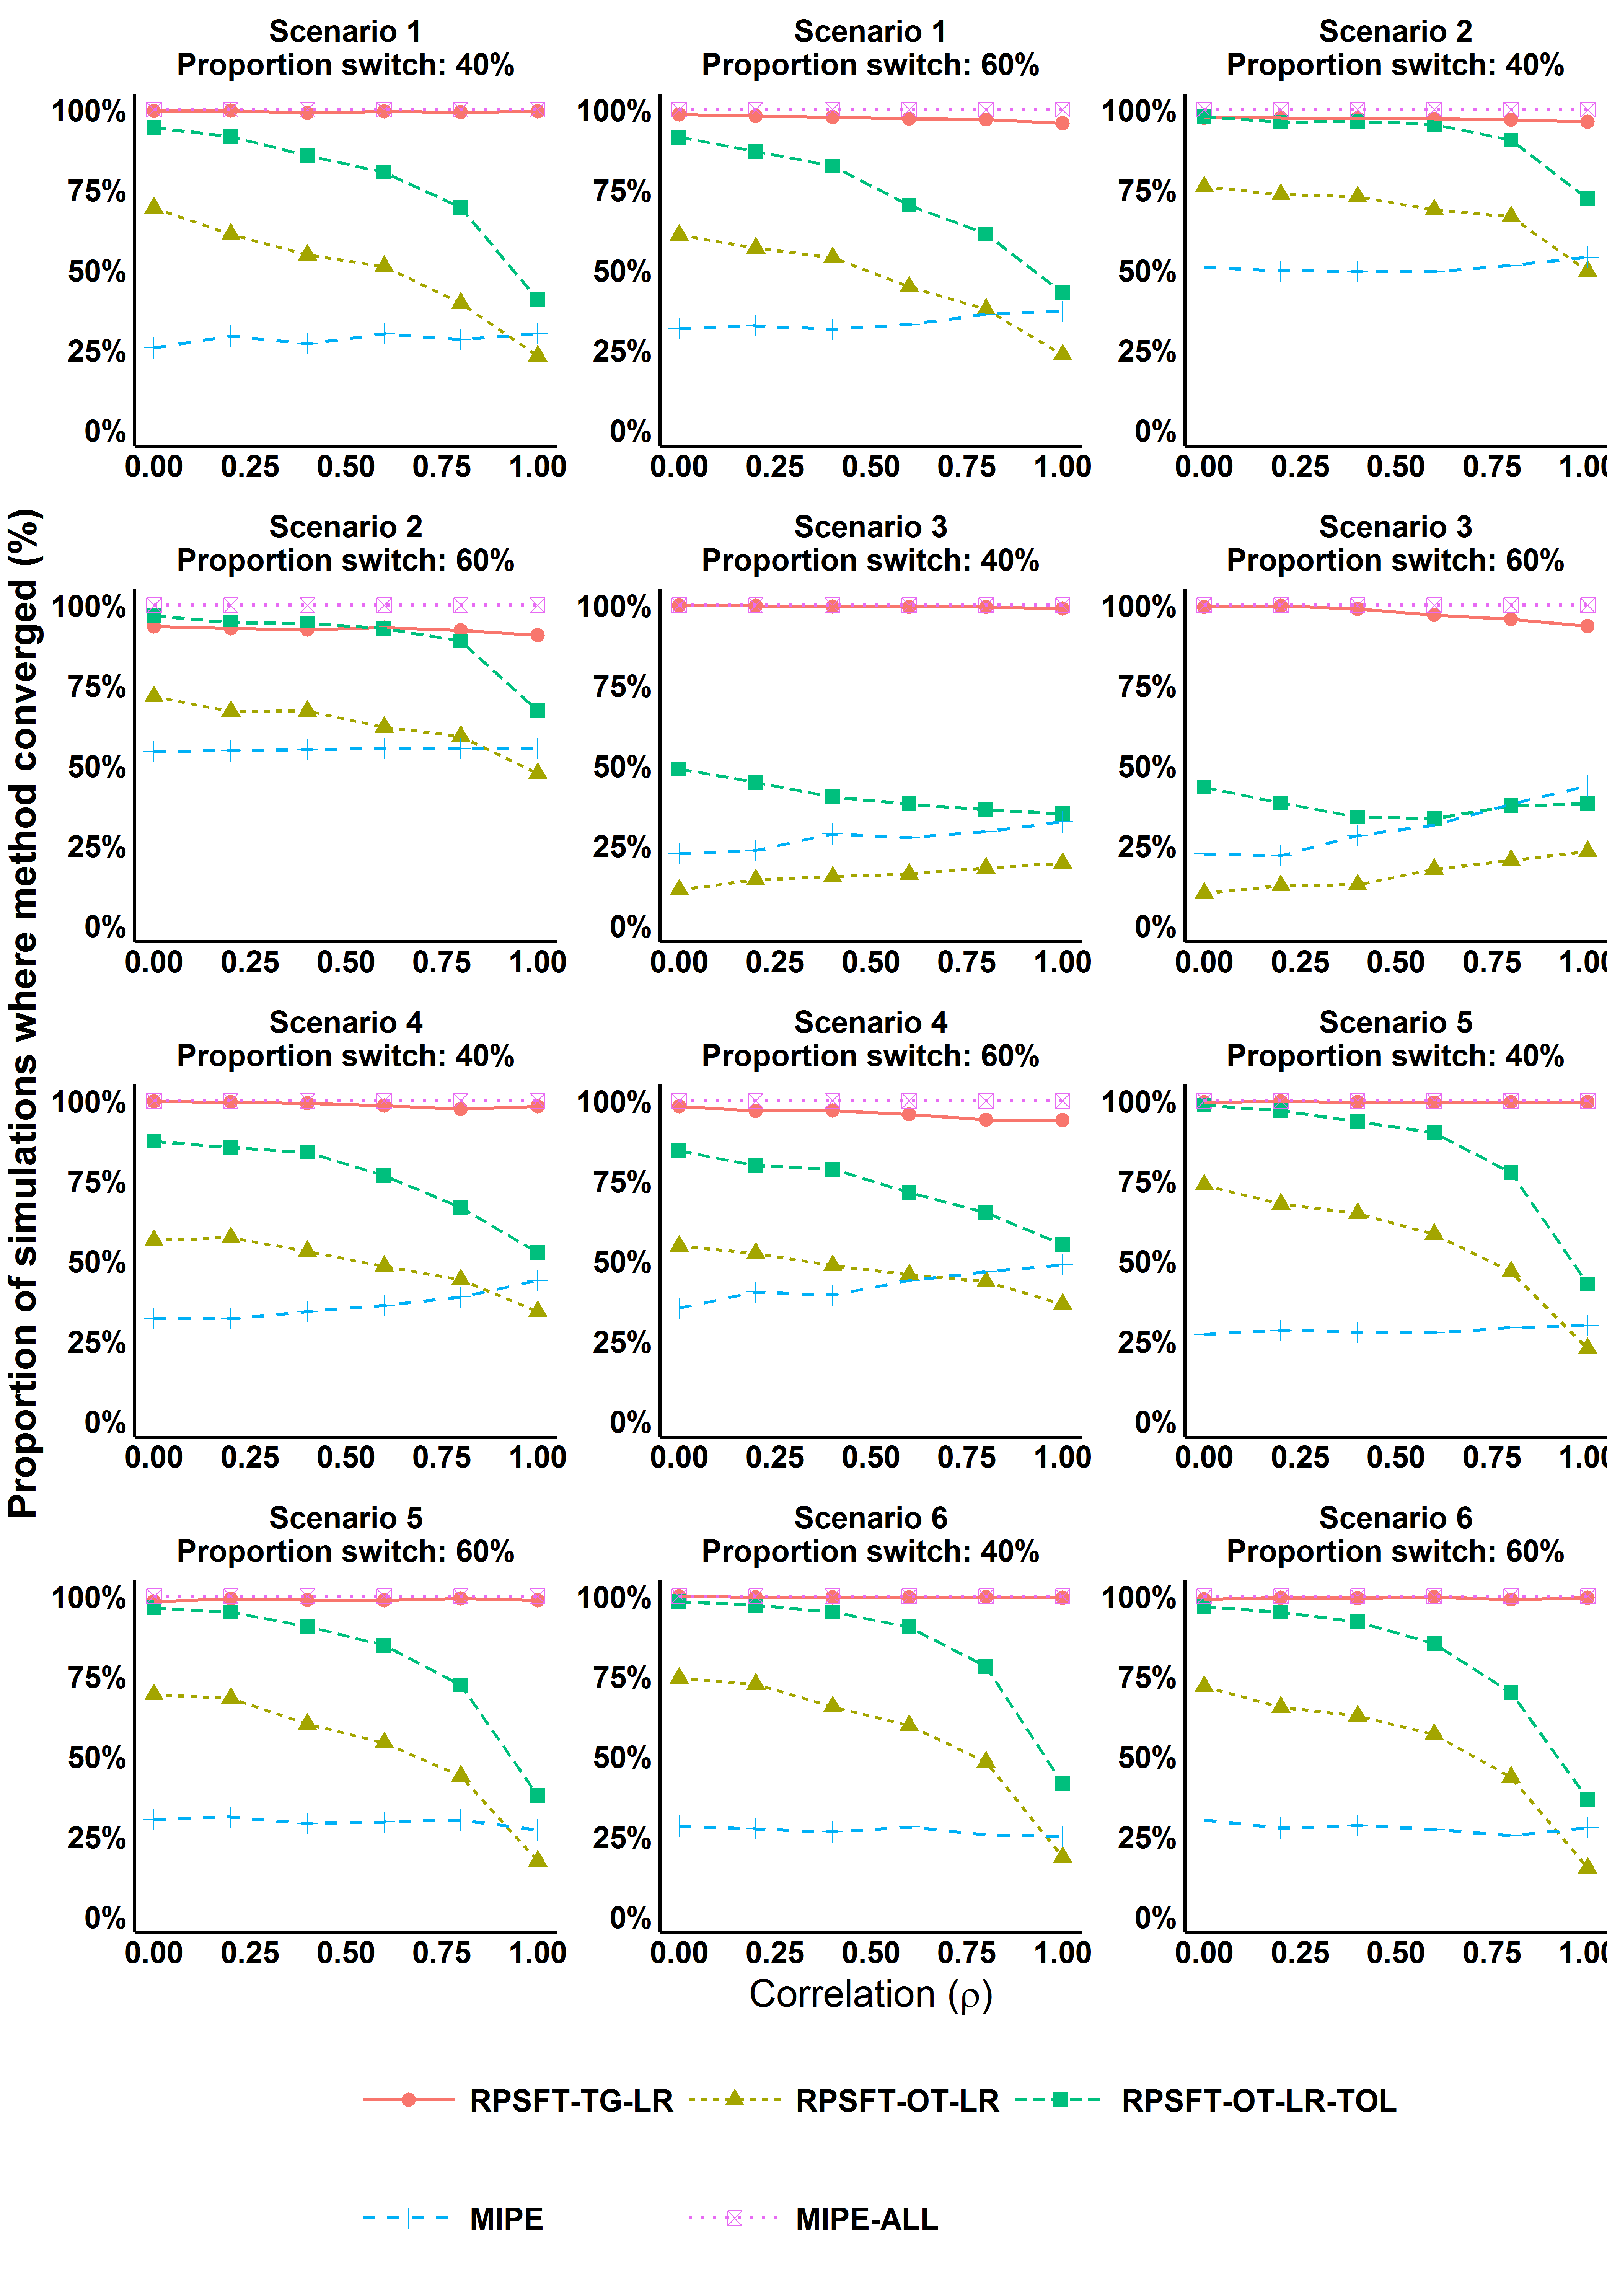
\includegraphics[width=13cm]{images/chap_sim3/comp_conv.png}
\caption{\label{F:chap_sim3:conv}  This figure shows the proportion of simulations where the complex methods rank-preserving structural failure time (RPSFT) and modified iterative parameter estimation (MIPE) converged to a unique solution. For RPSFT while convergence was acceptable in the ``treatment group'' approach (RPSFT-TG) for the ``on treatment'' approach (RPSFT-OT) the convergence was poor in the majority of scenarios particularly where correlation was high with the imputation approach only having limited improvement (RPSFT-OT-TOL) in these cases. The iterative parameter estimation (MIPE) approach performs much worse than the ``treatment group'' approach to RPSFT whose assumptions it shares and is also poor compared to the ``on treatment'' approach to RPSFT for the majority of scenarios. } 
\end{figure}

\clearpage


\subsection{Bias}

\subsubsection{Simple methods}

Figure \ref{F:chap_sim3:simple_bias} shows the bias for all the simple methods. The same patterns to the bias as seen in the previous simulation study are again apparent. For the per-protocol analysis excluding switch patients (PP-EX) there is again a large bias to overestimate the treatment effect regardless of correlation unless the time to progression is correlated perfectly with overall survival which is an implausible scenario. 

In the previous simulation study the Per-protocol Censoring at Switch (PP-CENS) analysis and the analysis including Treatment as a time-varying covariate (TVC and TVC2) were unbiased only when there was no correlation between time to progression and overall survival. In the scenarios investigated here this is again the case. It can be seen that the bias increases with increasing correlation between time to progression and overall survival. 

Across all the scenarios the ITT analysis underestimated the true treatment effect as expected. As seen previously the amount of bias is dependent on the magnitude of switch treatment effect so for scenarios 2 and 6 where the effect of switch treatment is minimal the ITT analysis shows less bias. This also explains to a certain extent the trend to decreasing bias with increasing correlation seen in scenario 3 as for this scenario the true treatment effect is also reduced with increasing correlation.

\begin{figure}[ht]
\centering
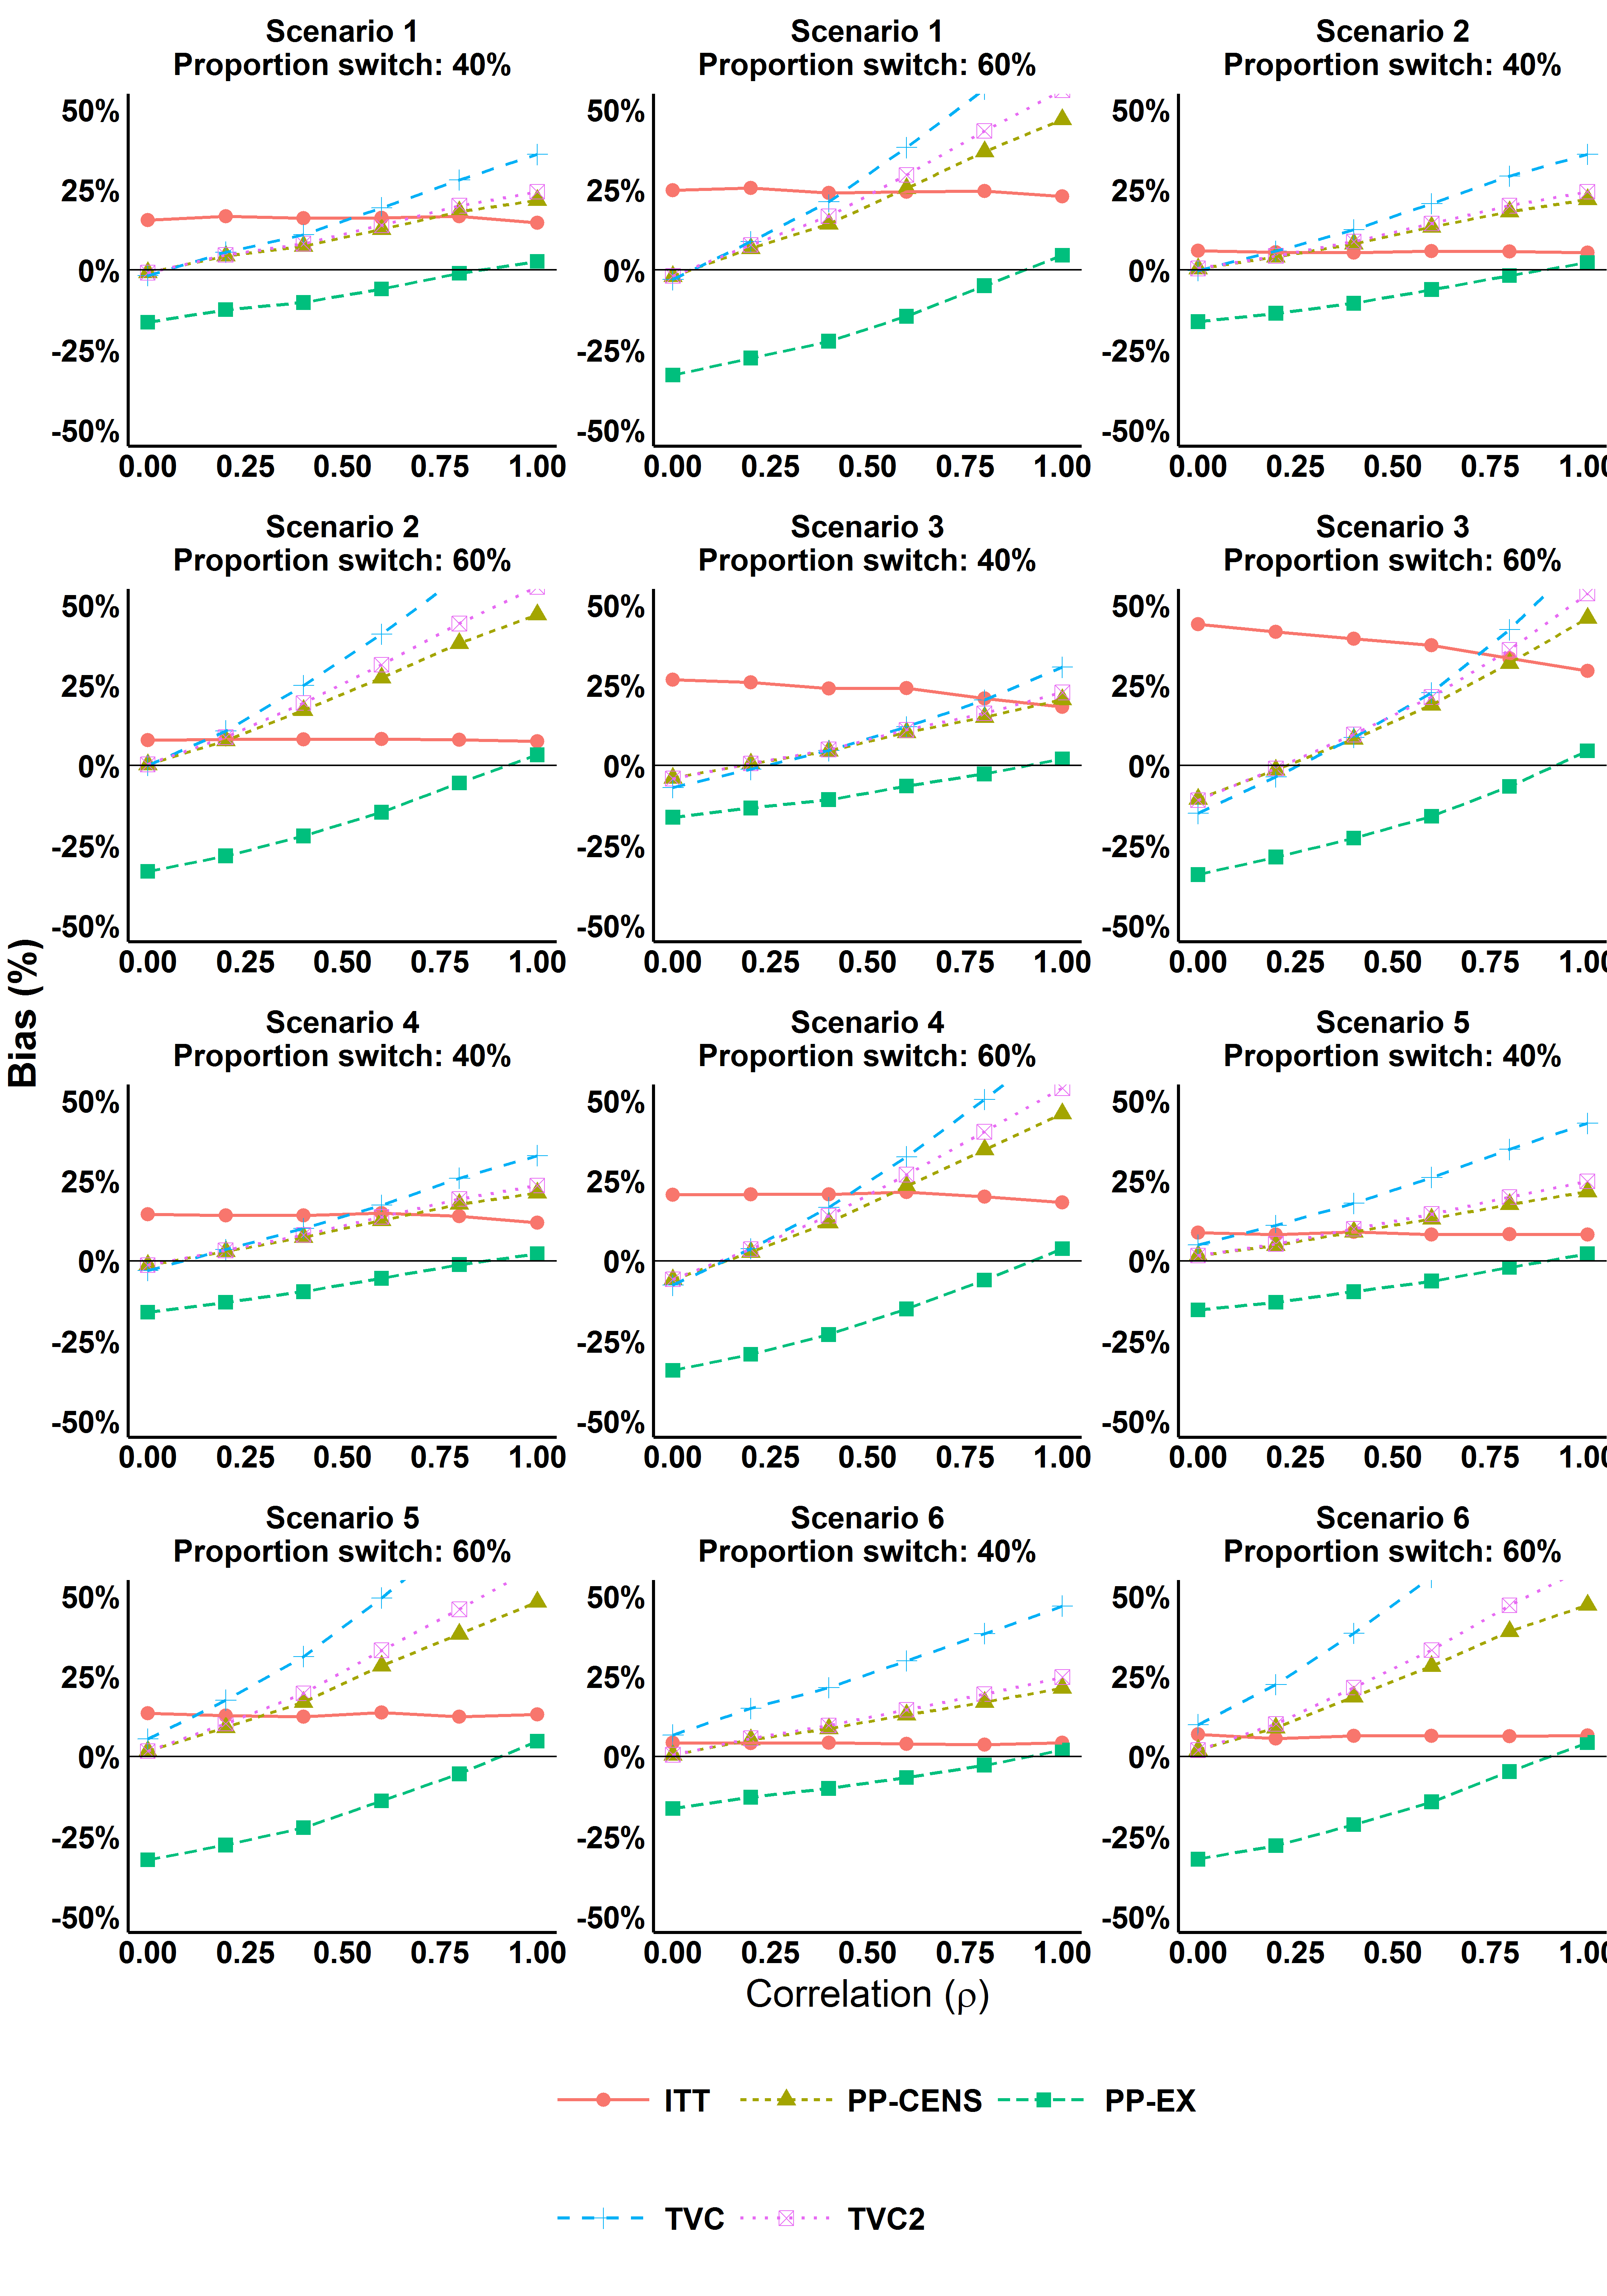
\includegraphics[width=13cm]{images/chap_sim3/simple_bias.png}
\caption{\label{F:chap_sim3:simple_bias} The bias for each of the simple methods in the scenarios for simulation study 2. For the Per-protocol Excluding Switch Patients (PP-EX) analysis the bias is large across all correlations. As with simulation study 1 for the Per-protocol Censoring at Switch (PP-CENS) analysis and the analysis including Treatment as a time-varying covariate (TVC and TVC2) there is reduced bias when there is no correlation between survival and time to progression but a very large bias otherwise. The ITT analysis consistently underestimates the true treatment effect across all scenarios mostly independently of correlation.} 
\end{figure}

\clearpage

\subsubsection{Complex methods}

Figure \ref{F:chap_sim3:comp_bias12} show the percentage bias for selected complex methods investigated in scenario 1 and 2. Compared to the simple methods the percentage bias is much reduced with the ``treatment group'' approach to RPSFT and two-stage AFT (2SAFT) performing the best. It is unclear why the iterative parameter estimation approach (MIPE) overestimates the treatment effect while the weibull model approach (MIPE-WEIB) simultaneously underestimates the treatment effect but performance is noticeably worse than the RPSFT approaches. 


For scenarios 3 and 4 the percentage bias is shown in Figure \ref{F:chap_sim3:comp_bias34} and the data generating mechanism could be expected to match closer to the assumptions of the ``on treatment'' approach to RPSFT with the treatment effect only applying during exposure to experimental treatment. Despite this the bias of this method and the bias of the ``treatment group'' approach are very similar with the ``treatment group'' approach having slightly lower bias for large correlations. In these scenarios there again seems to be limited benefit to using the IPE method compared to the RPSFT method with both approaches to estimating a hazard ratio using the MIPE approach having a greater range of bias compared to the RPSFT approaches. In these scenarios the two-stage AFT method performs relatively badly compared to the good performance elsewhere. To investigate this further Figure \ref{F:chap_sim3:2saft_bias34} shows the bias for the different implementations considered and it can be seen that for scenario 3 the bias can be improved by avoiding re-censoring (2SAFT-NC), however, this doesn't seem to be a universal fix as this increases the bias for scenario 4.

For scenarios 5 and 6 the bias of the RPSFT and MIPE methods is expected to be larger due to the violation of the common treatment effect assumption and as seen in Figure \ref{F:chap_sim3:comp_bias56} these methods do tend to overestimate the treatment effect here independently of correlation. Meanwhile the bias for the two-stage AFT method is very low across all these scenarios regardless of correlation with a maximum bias of 2.6\%.


\begin{figure}[ht]
\centering
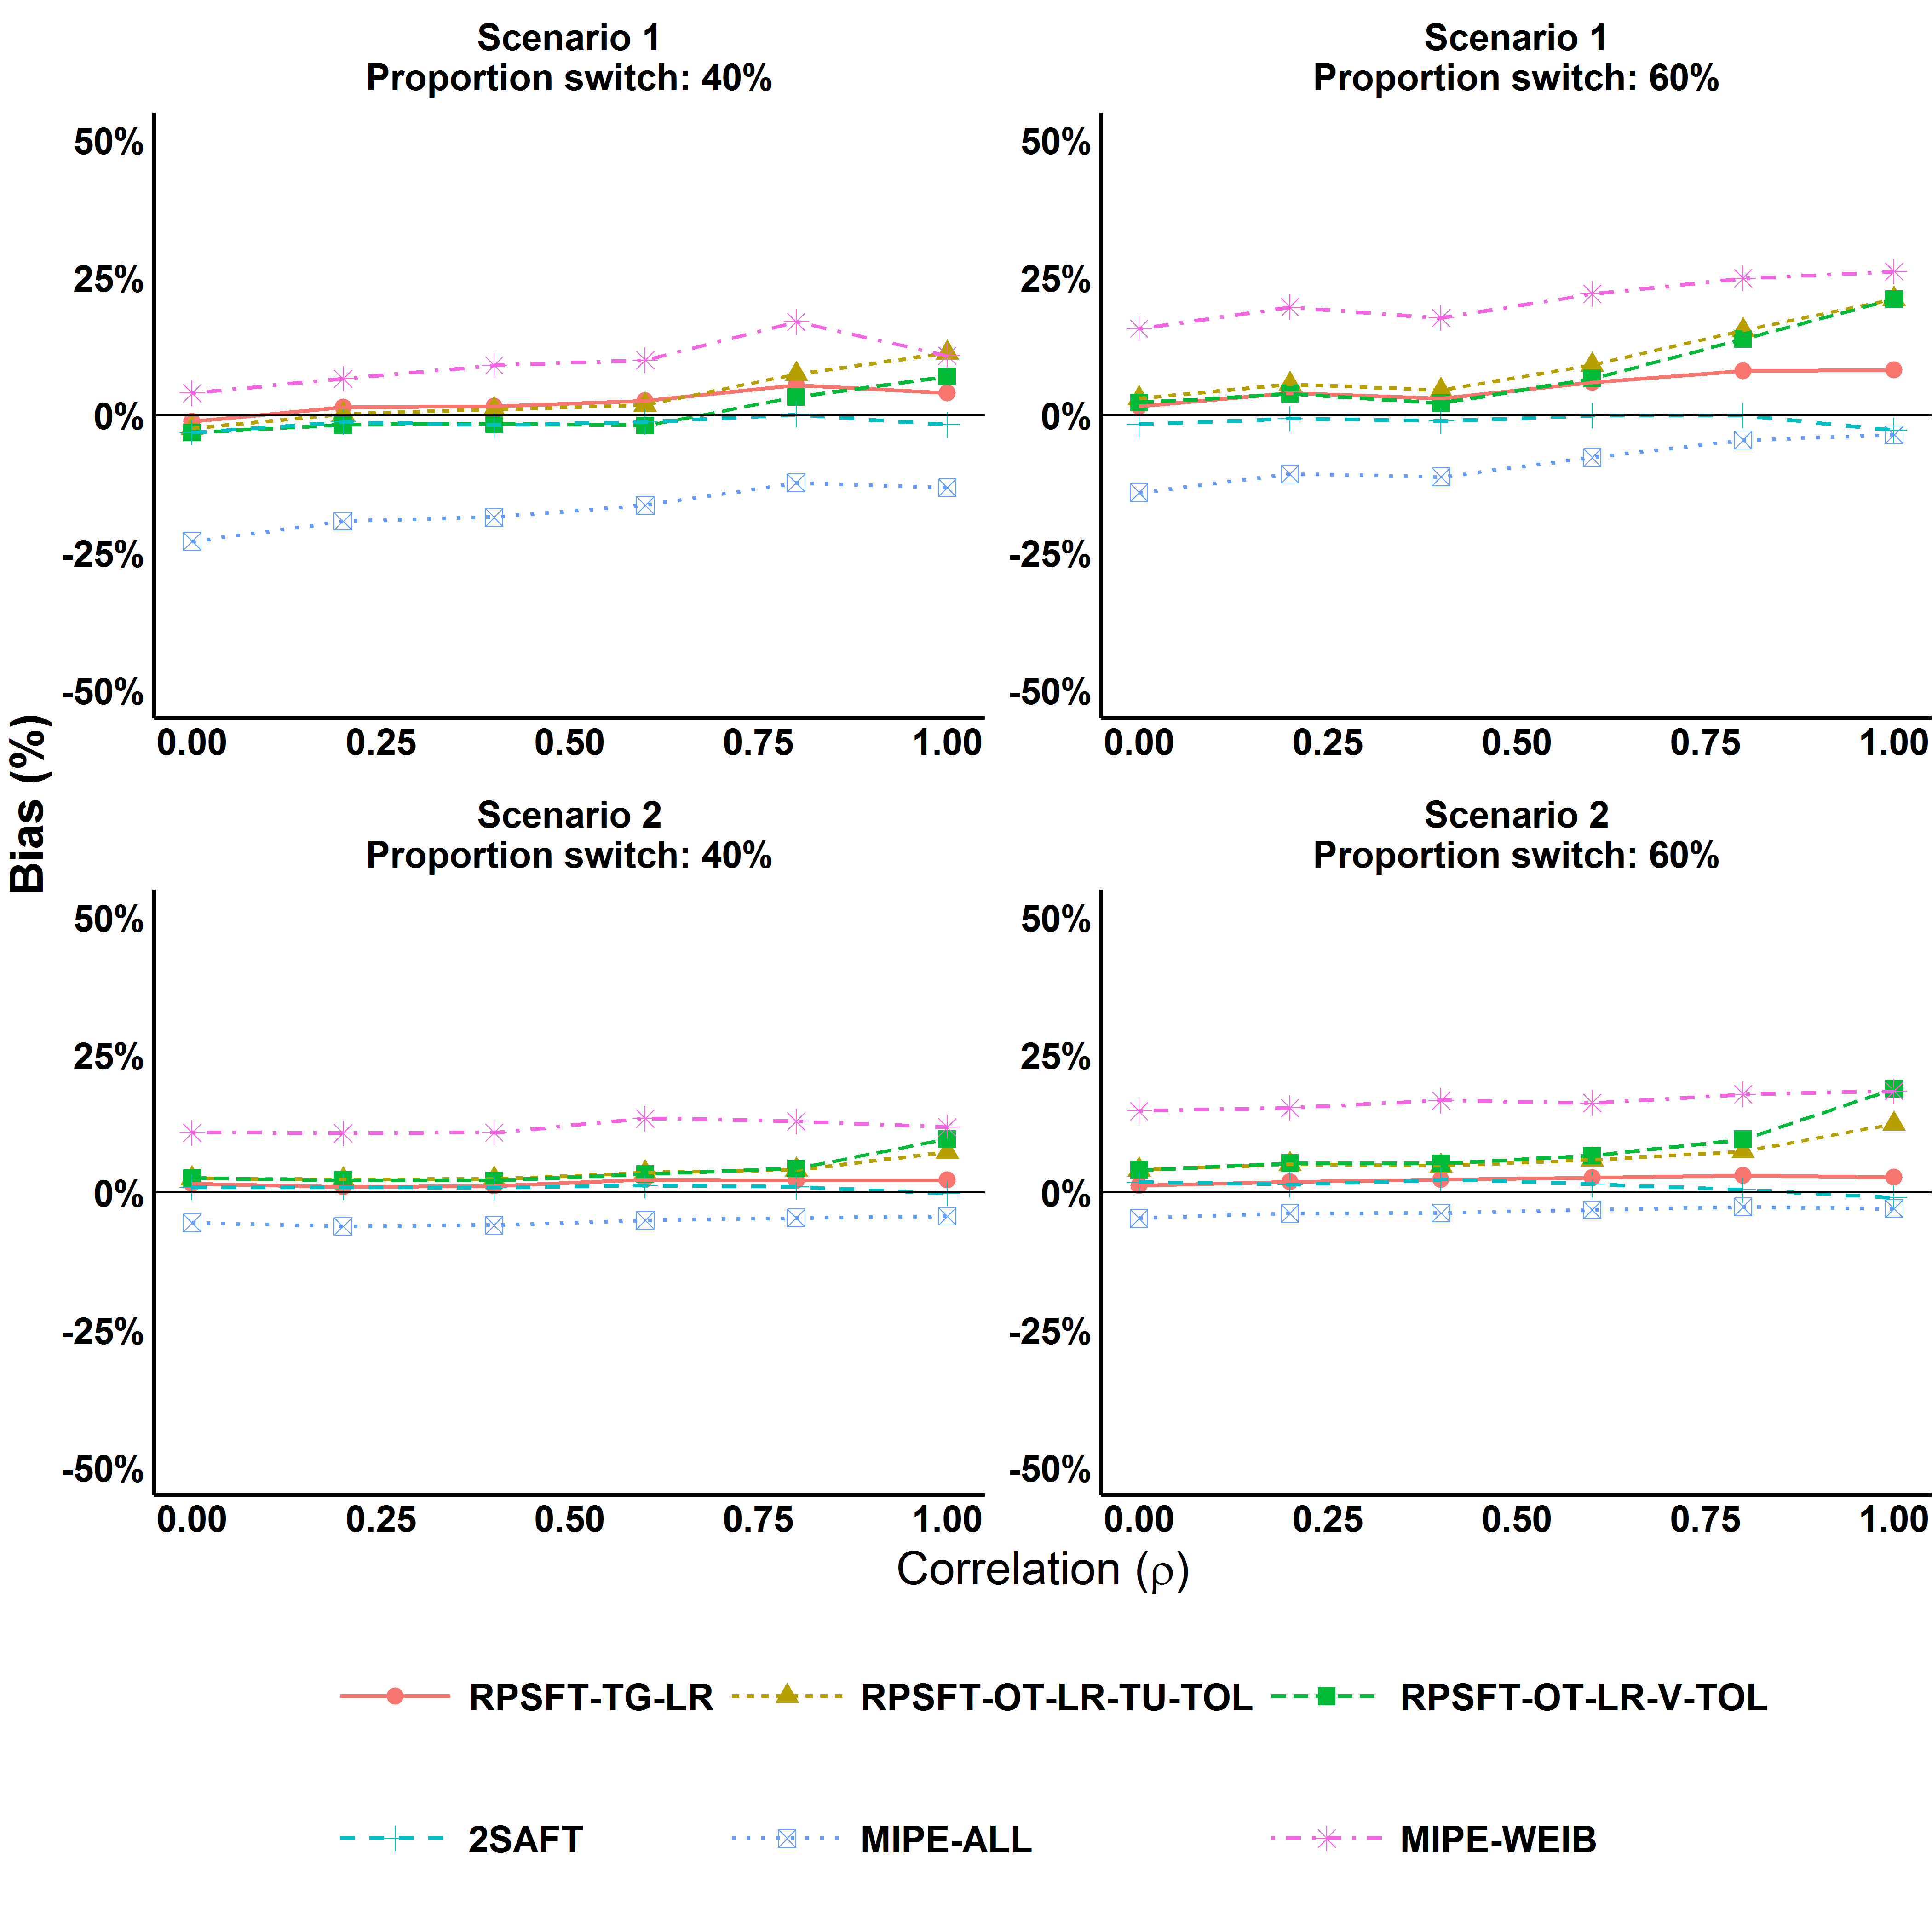
\includegraphics[width=13cm]{images/chap_sim3/comp_bias12.png}
\caption{\label{F:chap_sim3:comp_bias12} The bias for selected implementations of the complex methods for Scenario 1 and 2. In these scenarios there is a reduction in hazard during treatment and a reduced residual effect after treatment. For Scenario 1 the ``true''  hazard ratio is around 0.7 while for Scenario 2 it is approximately 0.9 as shown in Figure \ref{F:chap_sim3:truehr} which explains the lower bias seen in Scenario 2 compared to Scenario 1. In general the different approaches to RPSFT used here have a similar level of bias with the ``treatment group'' approach (RPSFT-TG) generally performing better though the increased bias for the ``on treatment'' approach (RPSFT-OT) seen with high correlations maybe partially due to the low convergence of this method in scenarios with $\rho \geq 0.8$. The two-stage AFT (2SAFT) including recensoring and progression free survival as a covariate has very low bias in these scenarios.}
\end{figure}

\begin{figure}[ht]
\centering
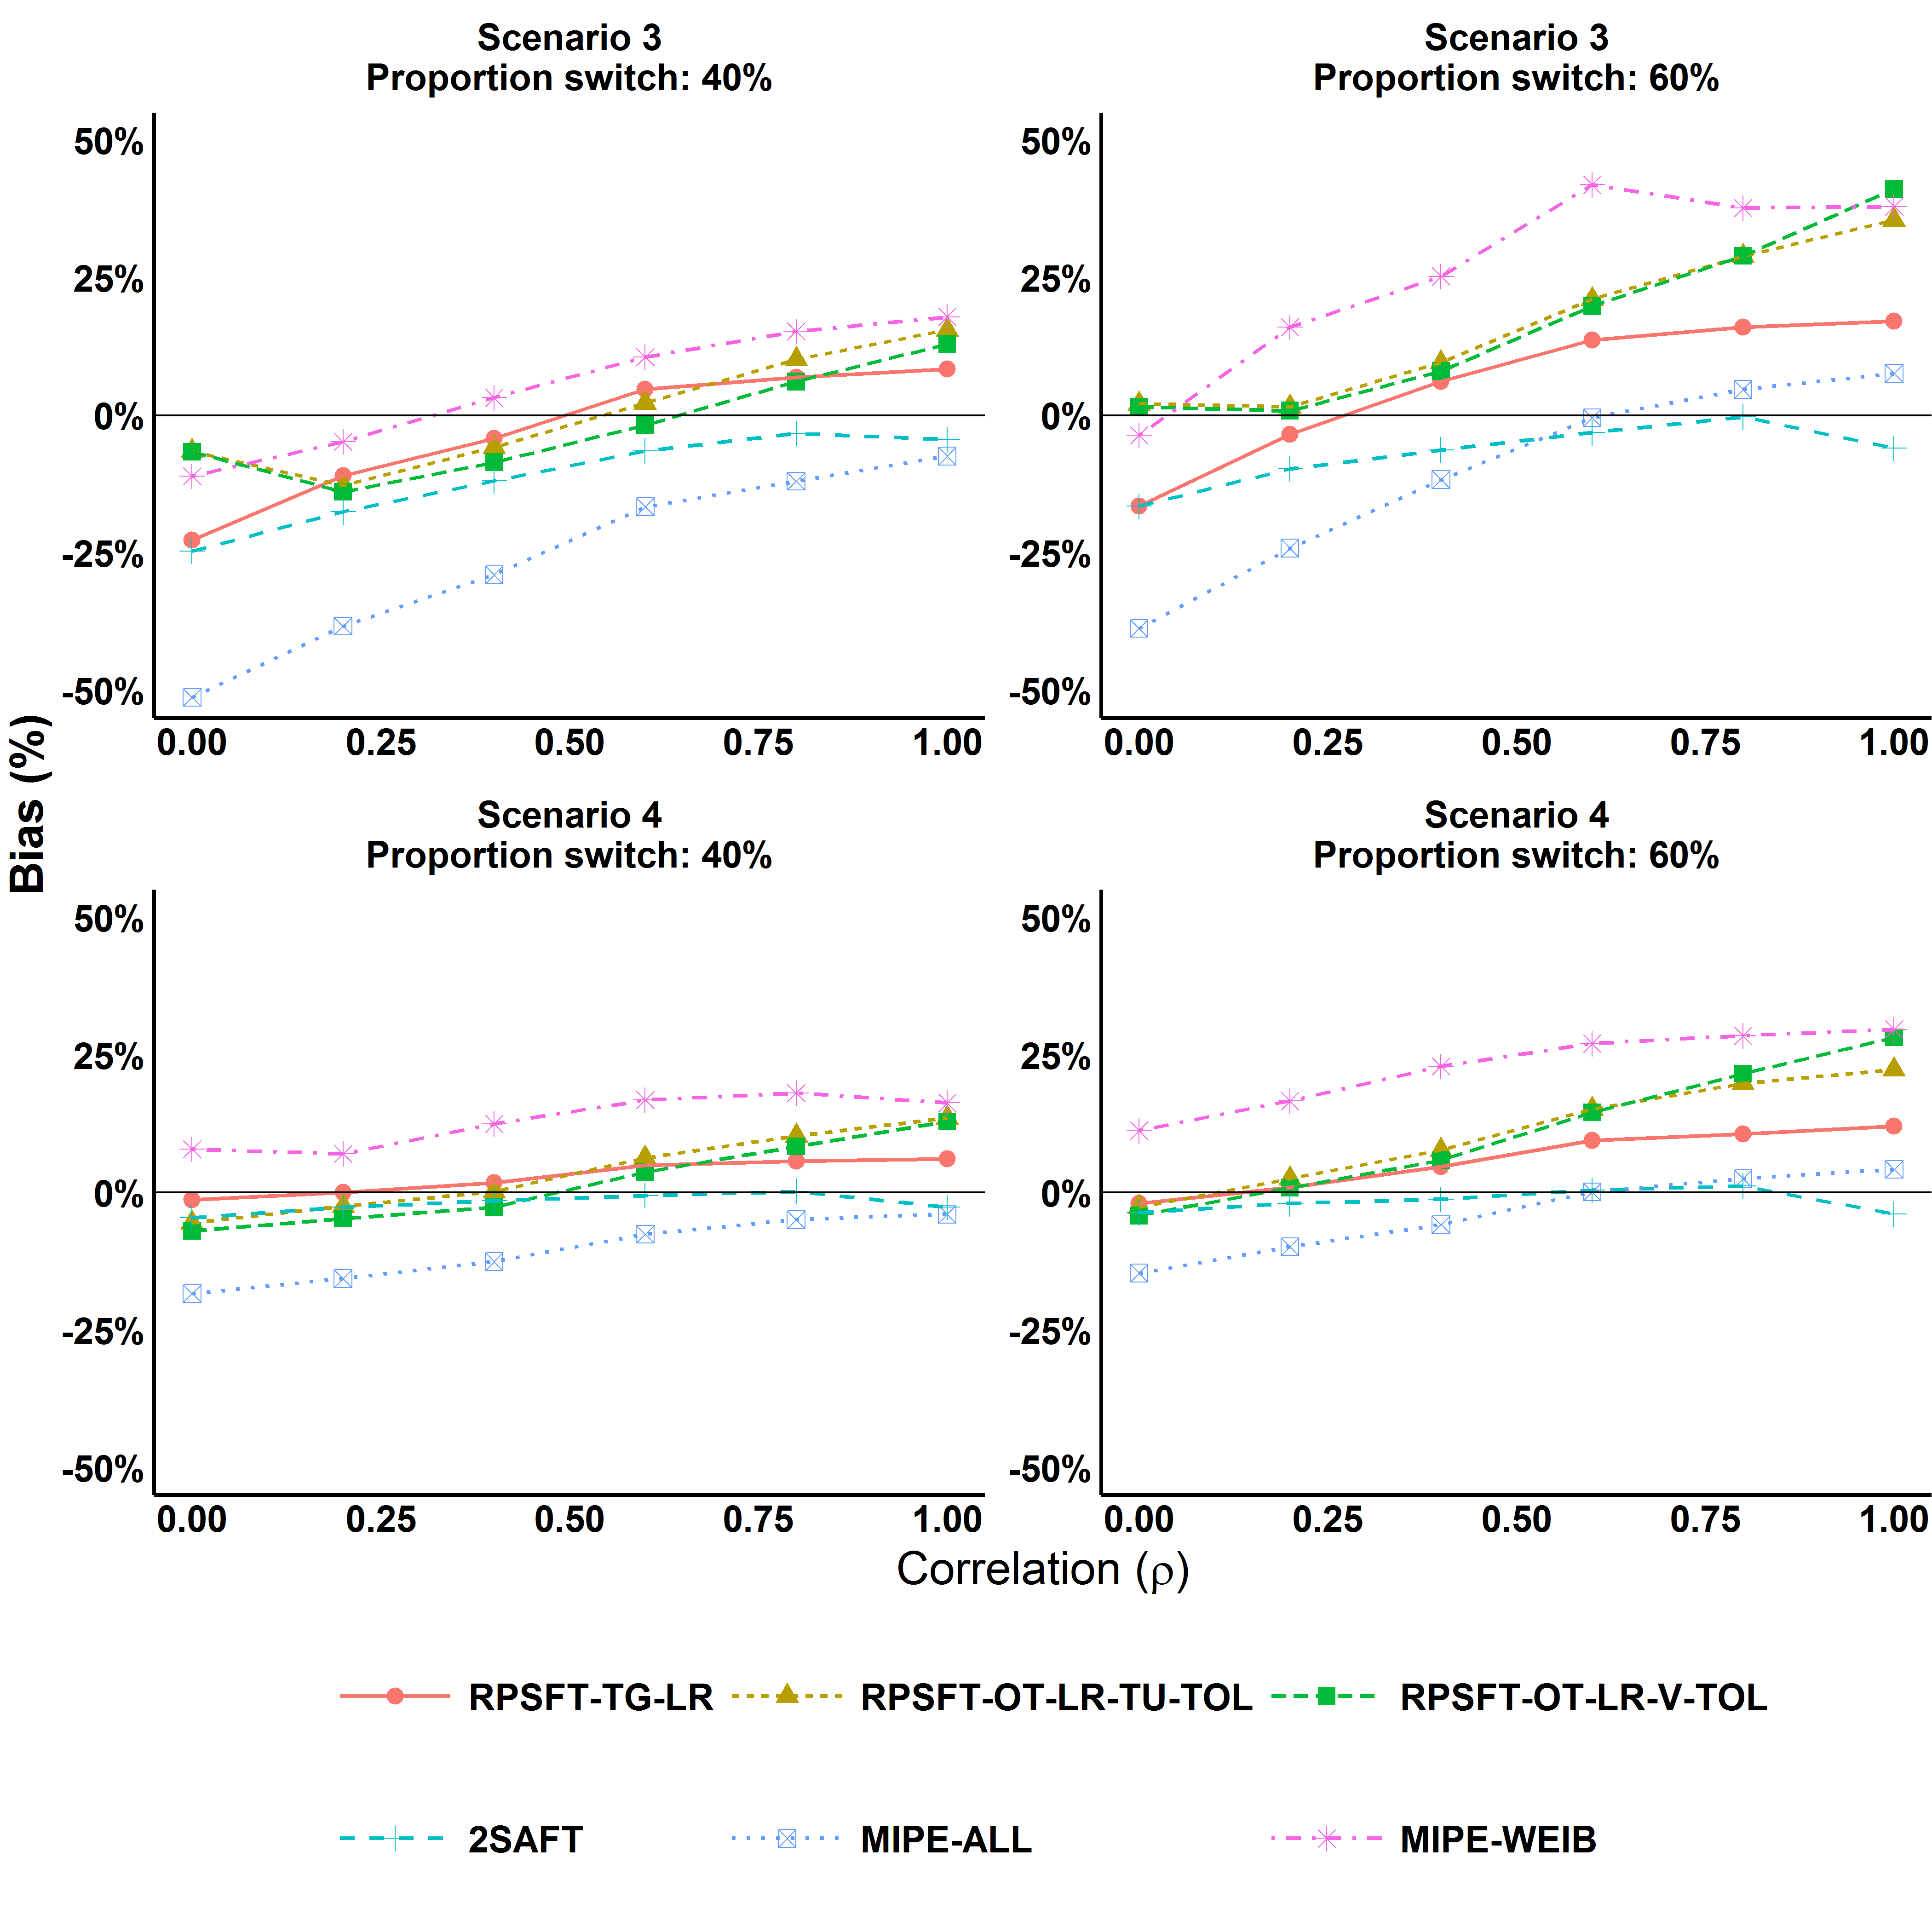
\includegraphics[width=12cm]{images/chap_sim3/comp_bias34.png}
\caption{\label{F:chap_sim3:comp_bias34} The bias for selected implementations of the complex methods for Scenario 3 and 4. In these scenarios the treatment is simulated to only reduce the risk of death during treatment. For the ``on treatment'' approach to RPSFT (RPSFT-OT-TOL) and the modified iterative parameter estimation using the weibull model (MIPE-WEIB) it should be noted that convergence is very low for Scenario 3. It was expected that the ``on treatment'' approach to RPSFT would perform better here as it is closer to the data generating mechanism, however, this does not appear to be the case with only a slight reduction in bias compared to the ``treatment group'' approach. Surprisingly the two-stage AFT (2SAFT) including recensoring and progression free survival as a covariate performs badly here with a few scenarios having greater bias than the RPSFT or MIPE methods. While it appears that there is some relationship between correlation and bias here this is somewhat hard to interpret as the ``true'' hazard ratio for these scenarios is also strongly related to correlation as shown in Figure \ref{F:chap_sim3:truehr}.} 
\end{figure}


\begin{figure}[ht]
\centering
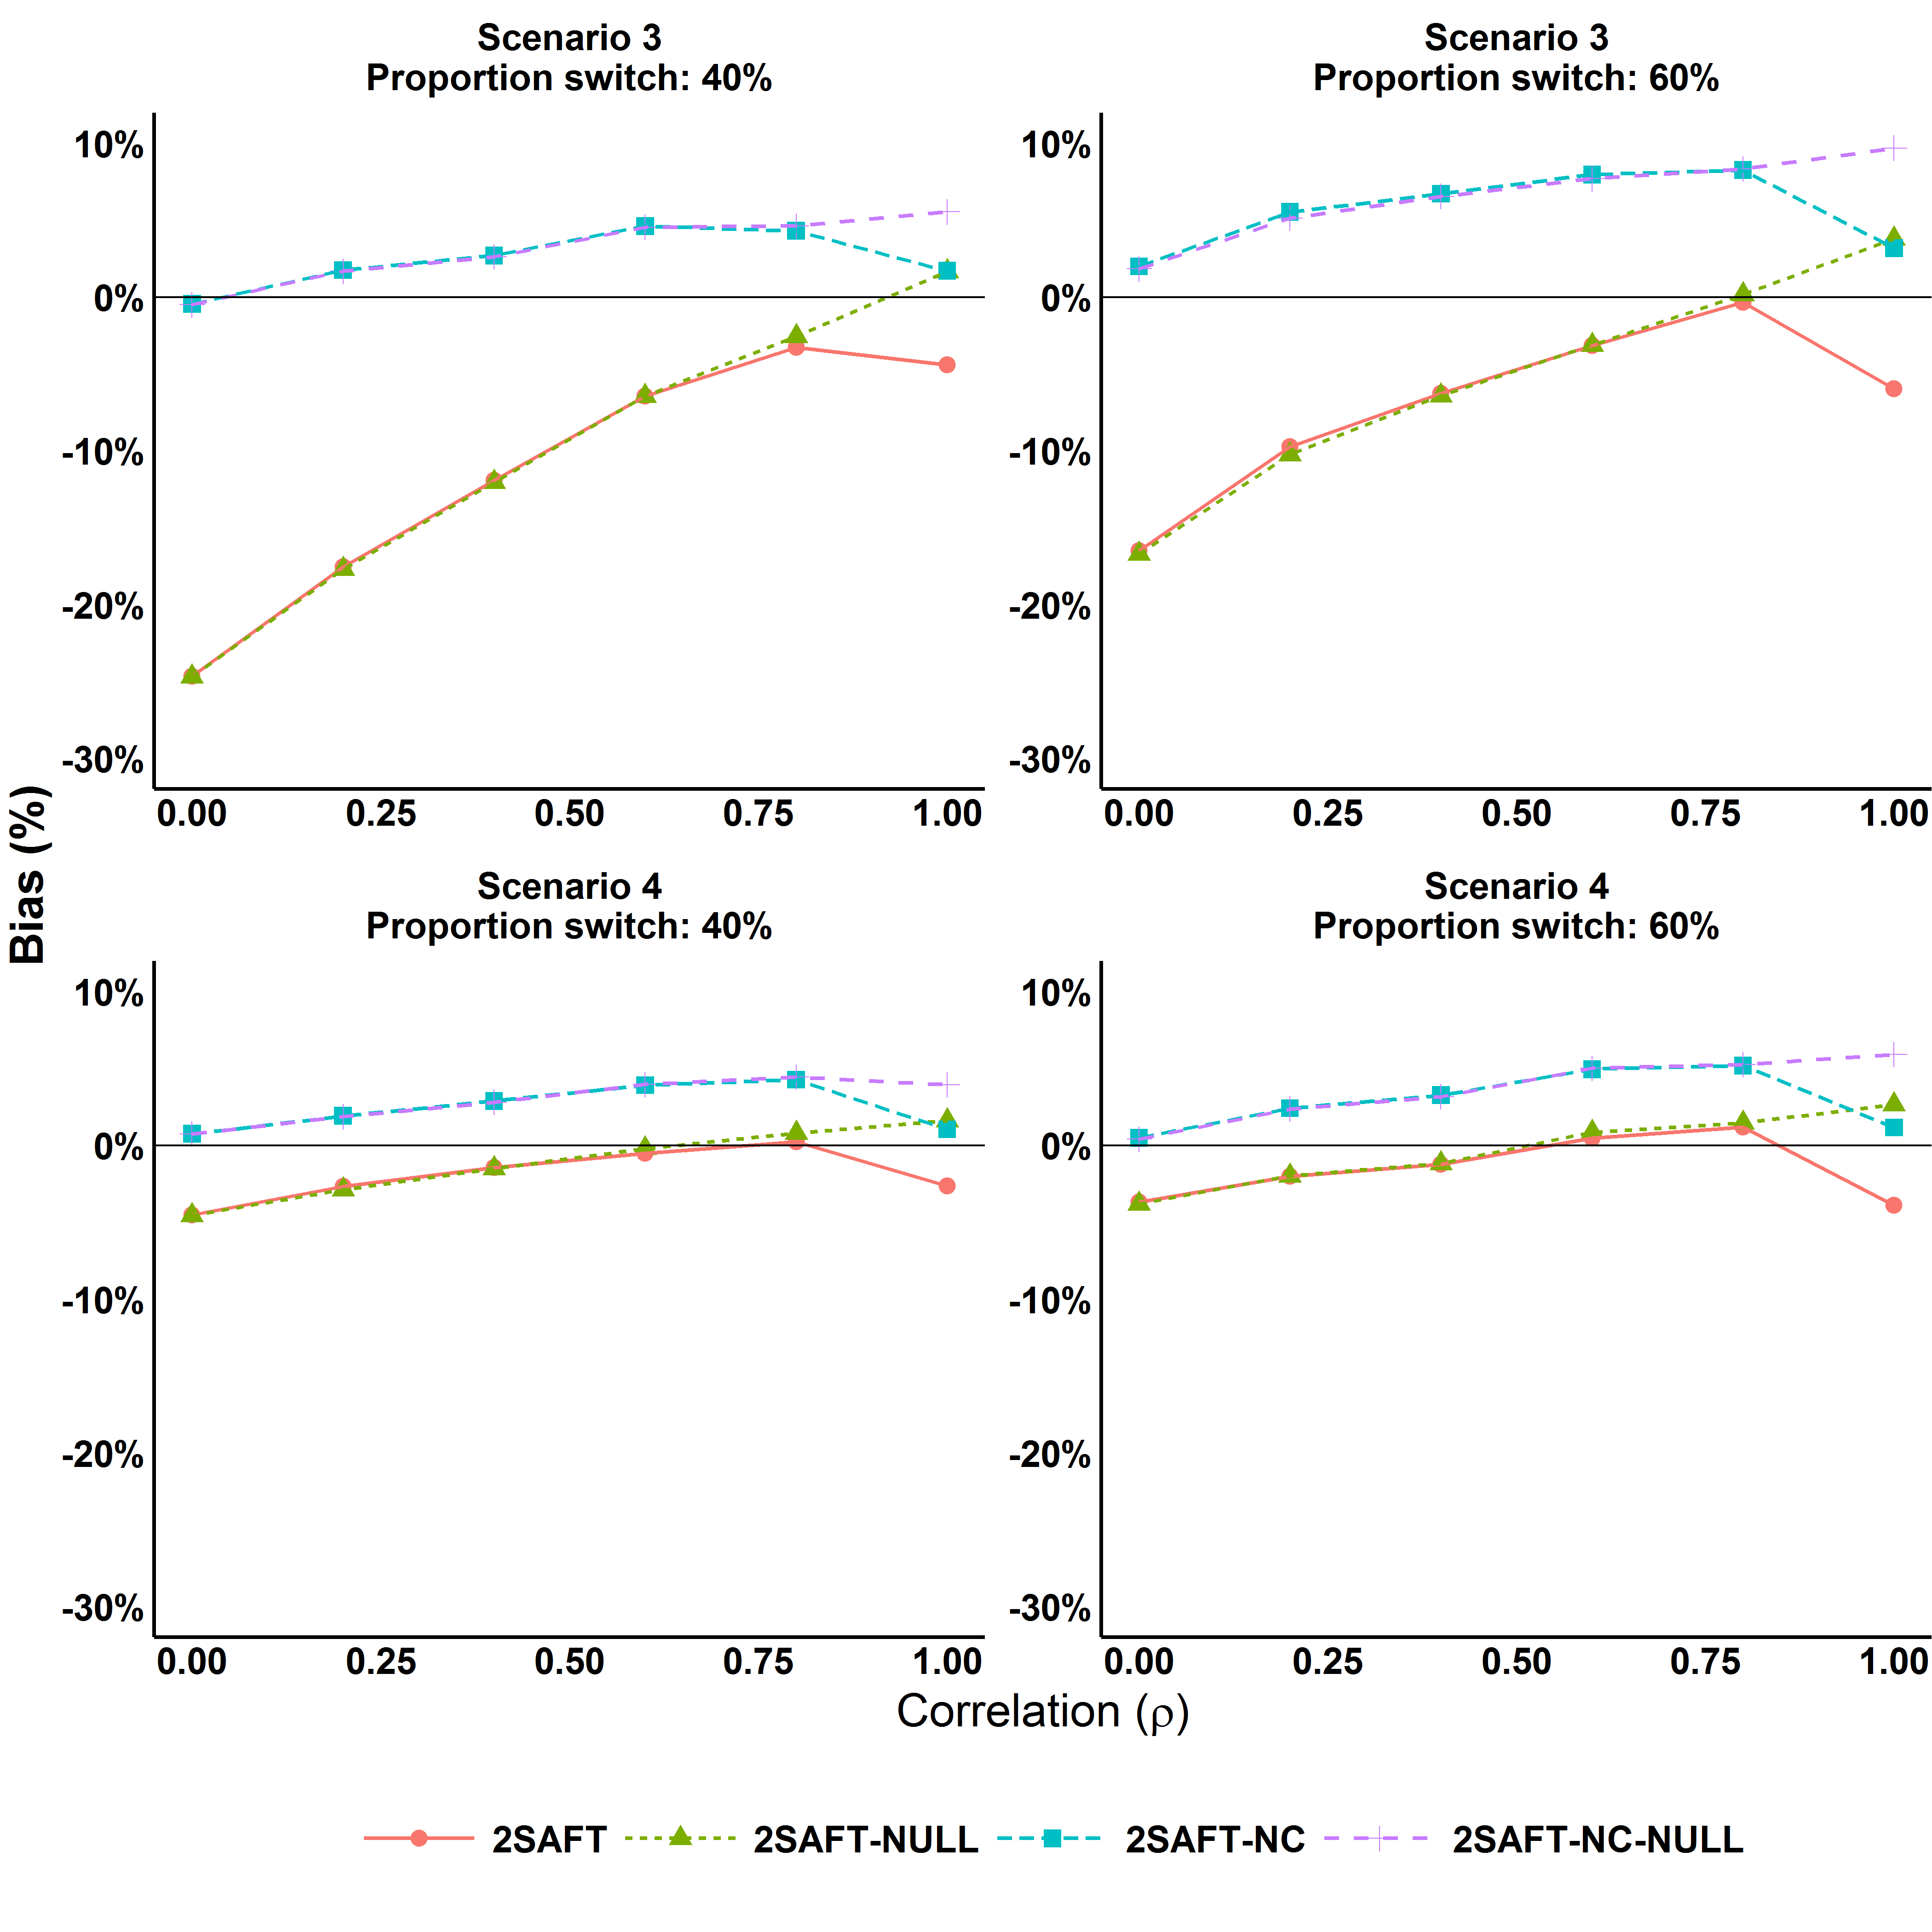
\includegraphics[width=12cm]{images/chap_sim3/2saft_bias.png}
\caption{\label{F:chap_sim3:2saft_bias34} The bias for all implementations of two-stage AFT model investigated for Scenario 3 and 4. In these scenarios the treatment is simulated to only reduce the risk of death during treatment. For scenario 3 it can be seen that the inclusion of a covariate for PFS into the model (2SAFT) or not (2SAFT-NULL) has negligible impact on the bias for the method compared to the reduction in bias when no-recensoring is performed (2SAFT-NC) and (2SAFT-NC-NULL).} 
\end{figure}


\begin{figure}[ht]
\centering
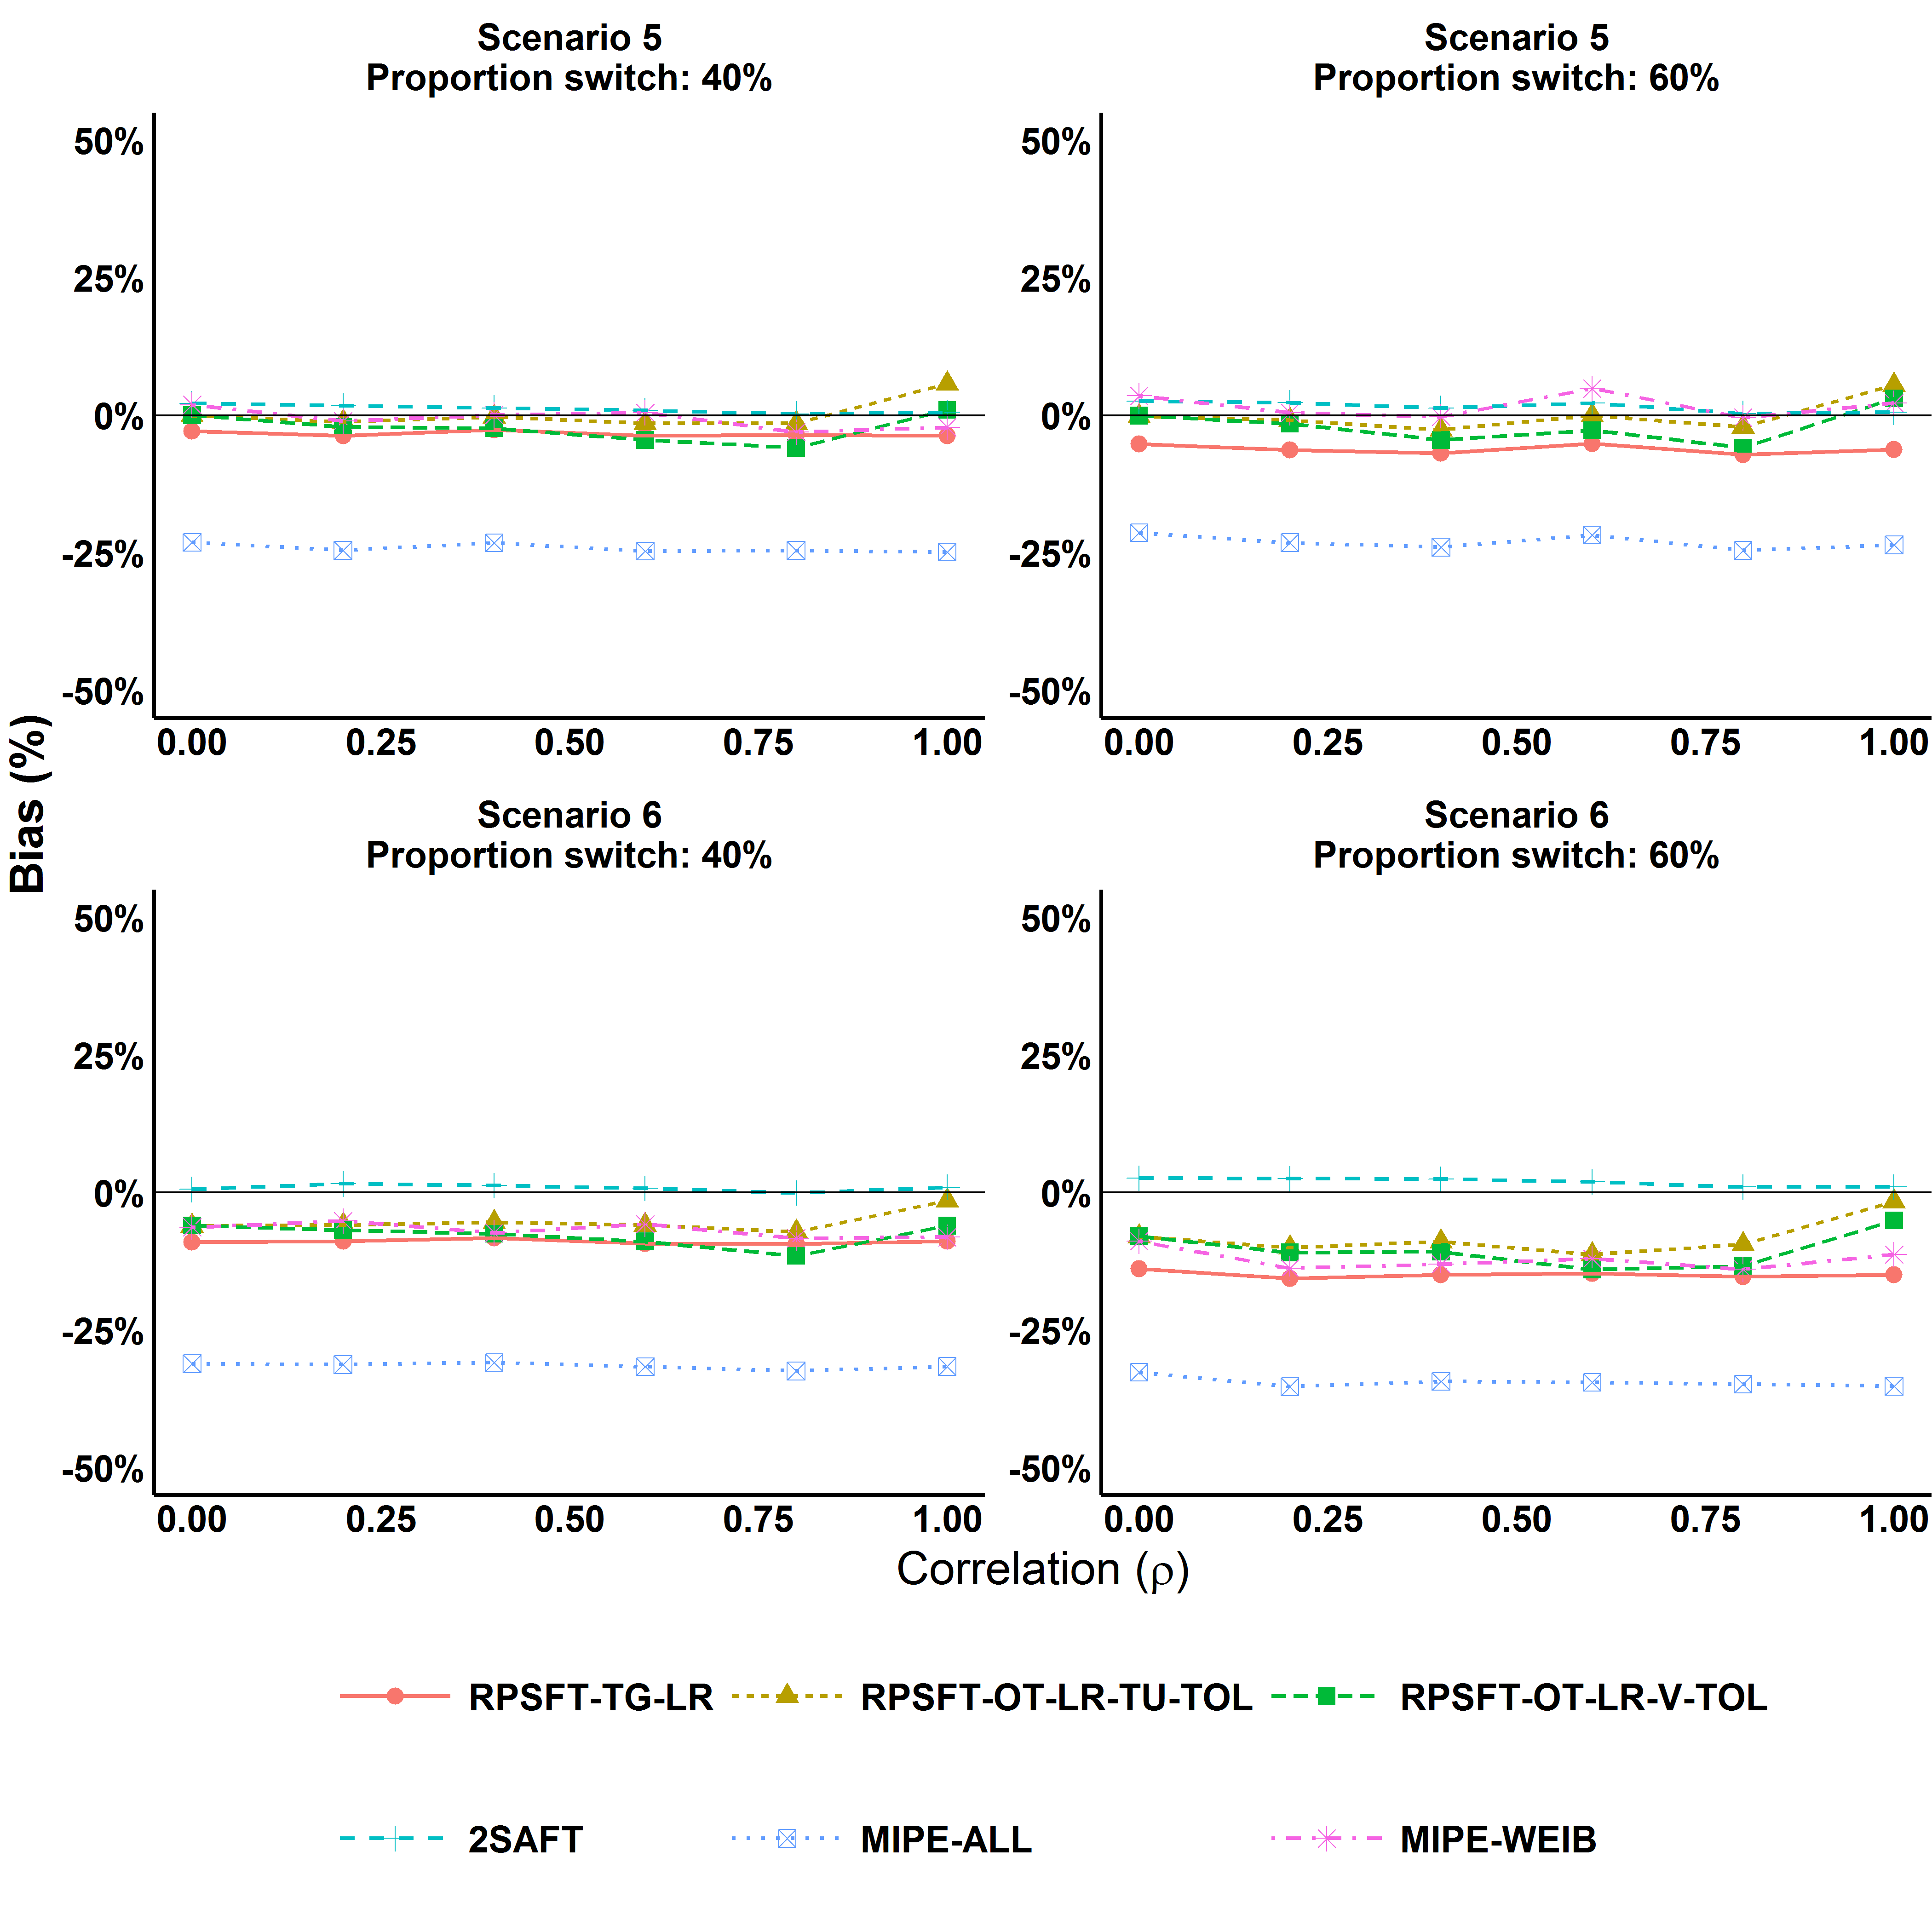
\includegraphics[width=12cm]{images/chap_sim3/comp_bias56.png}
\caption{\label{F:chap_sim3:comp_bias56} The bias for selected implementations of the complex methods for Scenario 5 and 6. In these scenarios the reduction in risk of death for switch treatment is reduced compared to the effect received as randomized treatment. As expected the rank-preserving structural failure time (RPSFT) and modified iterative parameter estimation (MIPE) methods show greater bias here than seen in the equivalent scenarios in the previous simulation study. The MIPE in general has greater bias than the RPSFT methods while the two-stage AFT (2SAFT) including recensoring and progression free survival as a covariate works well here with minimal bias.} 
\end{figure}

\clearpage

\subsection{Coverage}

Figure \ref{F:chap_sim3:simple_cov} and Figure \ref{F:chap_sim3:comp_cov} show the coverage of the confidence intervals estimated using from the simple methods and complex methods respectively. For the simple methods the coverage is very poor for the majority of the scenarios. For the RPSFT methods the correction to the confidence intervals as described in Section \ref{S:chap_methrev:RPSFTestHR} mean coverage is reasonable but not perfect. As expected the coverage for confidence intervals estimated using the MIPE method are poor and as noted by \cite{Zhang2016} there is a need for bootstrapping.

\begin{figure}[ht]
\centering
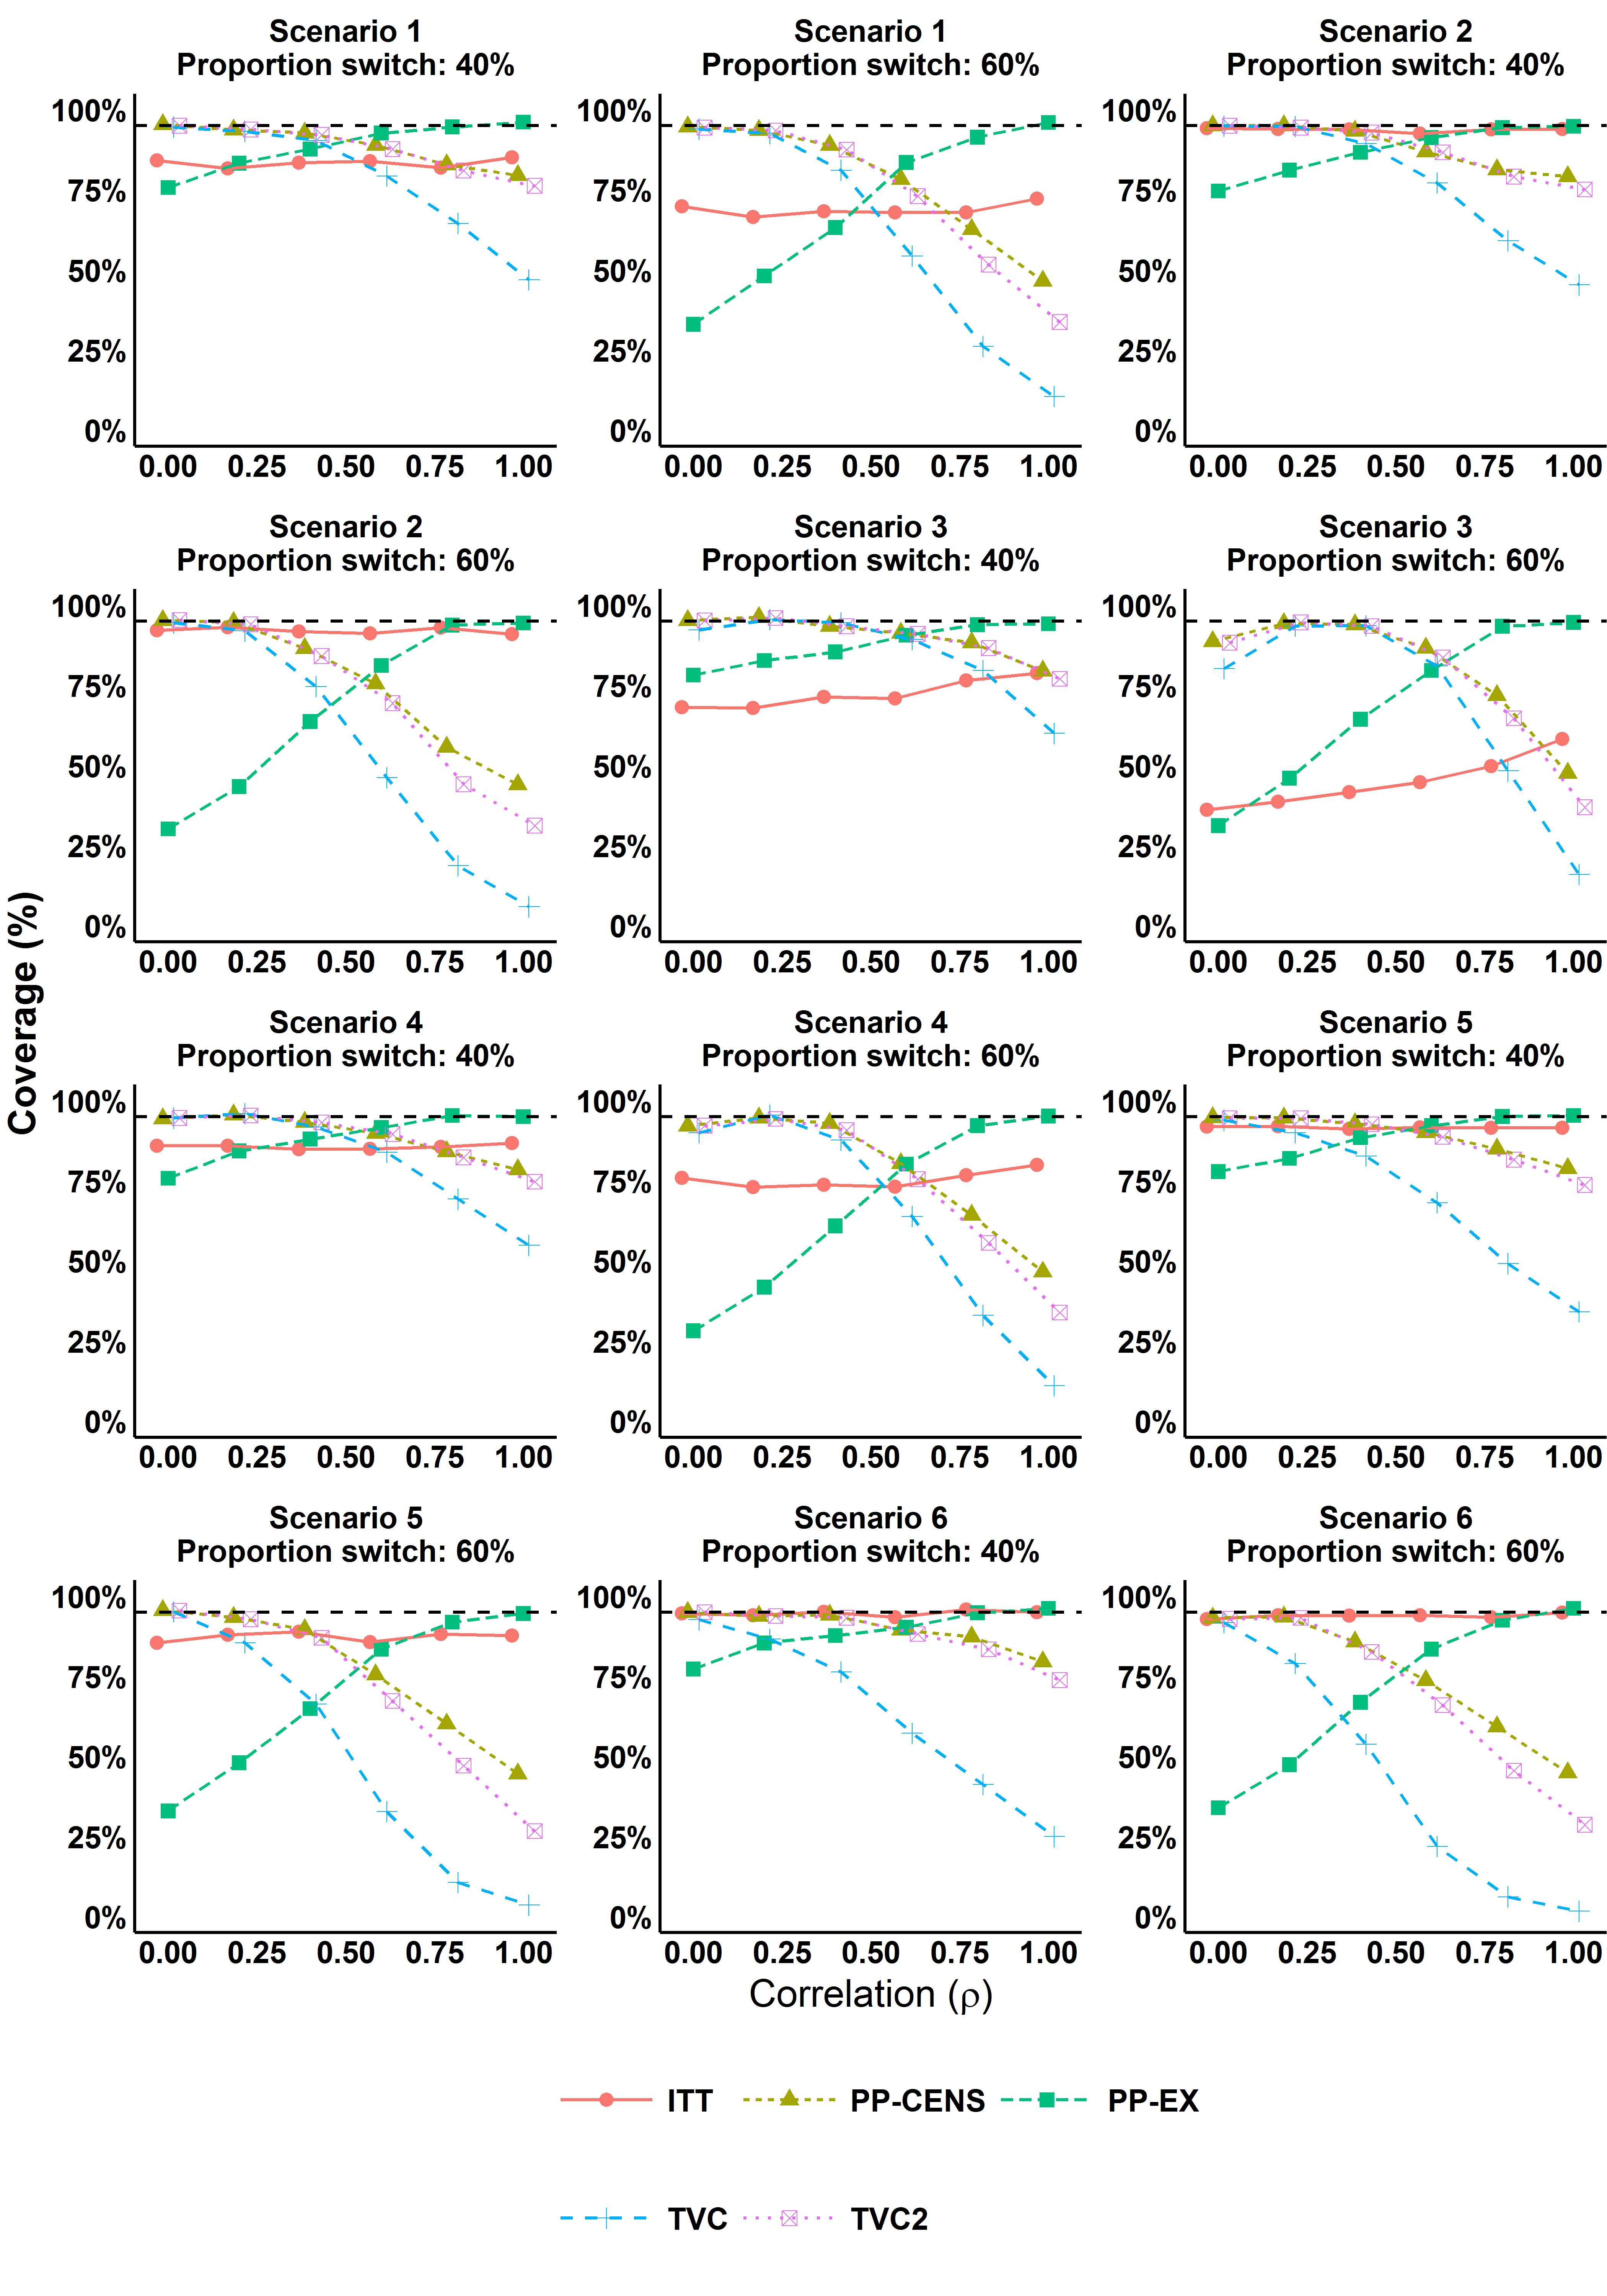
\includegraphics[width=13cm]{images/chap_sim3/simple_cov.png}
\caption{\label{F:chap_sim3:simple_cov} The coverage of the simple methods in this simulation study. The ITT performs reasonably here with a minimal coverage for the nominal 95\% confidence interval of 74.5\% that is mostly independent of correlation between time to progression and overall survival. The other methods such as treatment as a time varying covariate (TVC and TVC2) and the per-protocol analysis (PP-CENS) and (PP-EX) perform poorly. } 
\end{figure}

\begin{figure}[ht]
\centering
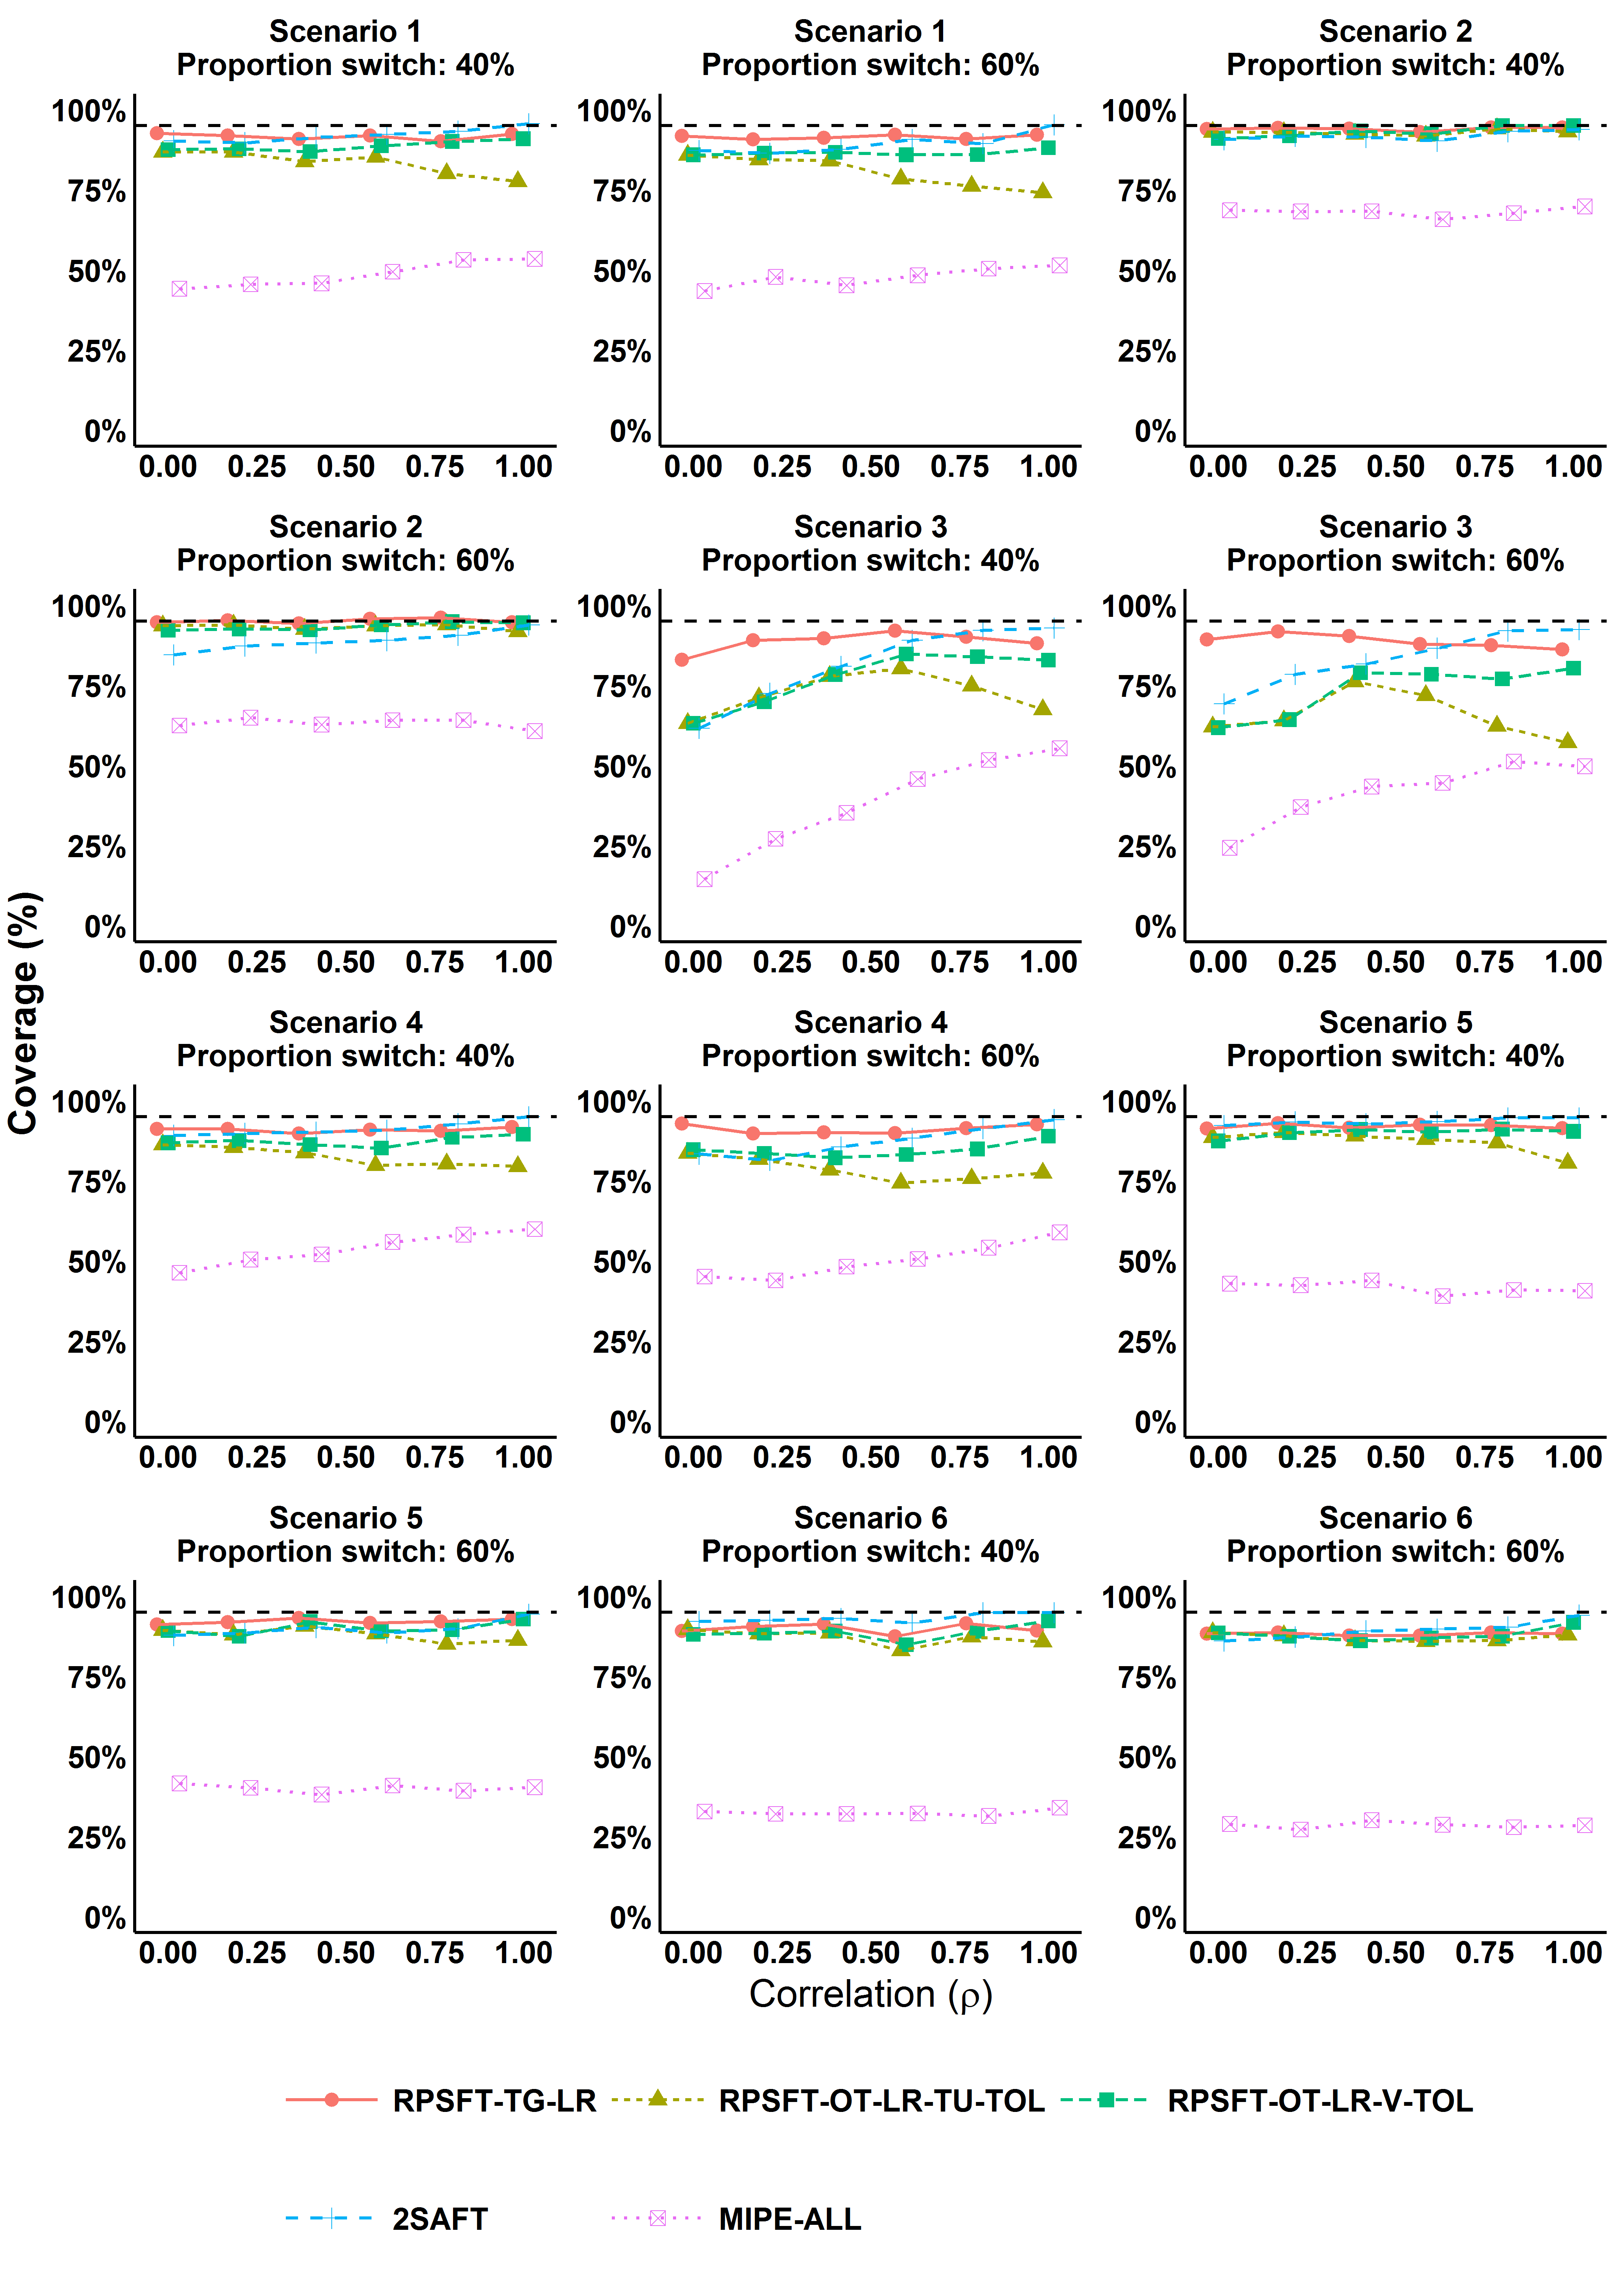
\includegraphics[width=13cm]{images/chap_sim3/comp_cov.png}
\caption{\label{F:chap_sim3:comp_cov} The coverage of the complex methods in this simulation study. For the majority of scenarios the coverage of confidence intervals for the ``treatment group'' approach to RPSFT (RPSFT-TG) using the test based correction of \cite{White1999} is acceptable. For the other RPSFT methods coverage is also reasonable but reduced relative to the ``treatment group'' approach. As expected confidence intervals for the iterative parameter estimate (MIPE) analysis have poor coverage and bootstrapping is clearly needed.} 
\end{figure}


\clearpage

\section{Conclusions of Simulation Study 2}

In this simulation study more complex patterns of treatment effect were investigated but the conclusions are very similar to those of the previous simulation study. For the per-protocol censoring at switch (PP-CENS) and both variations of treatment as a time-varying covariate (TVC and TVC2) unless there is no correlation between time to progression and overall survival the estimates of treatment effect show considerable bias. As expected the ITT analysis underestimated the treatment effect that would have been observed without switch across every scenario. The magnitude of bias depends on the magnitude of switch treatment effect with scenarios with a smaller treatment effect having smaller bias.

The two-stage AFT (2SAFT) method performs well across the majority of the 72 scenarios investigated except for a handful of the scenarios where the treatment is simulated to only have a reduction on the risk of overall survival during treatment exposure. It is unclear what causes this but it appears that it may partially be related to censoring on the counterfactual time scale.

In general the ``treatment group'' (RPSFT-TG) approach performed the best of the various flavours of RPSFT investigated with negligible differences compared to the ``on treatment'' (RPSFT-OT) approach even in scenarios that should match better to the assumptions of that model. This may be related to the convergence of the ``on treatment'' approach as the scenarios where bias was increased compared to the ``treatment group'' approach were also scenarios where the convergence was very poor for the ``on treatment'' approach. Finally even for the scenarios with a reduced effect of switch treatment violating the common treatment effect the bias was increased but not dramatically when compared to the bias observed with the simple methods. 

Once again though the value of the MIPE approach seems very limited as the bias was in some scenarios larger than observed with the RPSFT and the fact that  the convergence is worse than the ``treatment group'' approach to RPSFT and often worse than the ``on treatment'' approach suggests this method adds few benefits given the need to make additional parametric assumptions.




